\documentclass[10pt]{article}
\usepackage[utf8]{inputenc}
\usepackage[T1]{fontenc}
\usepackage{graphicx}
\usepackage[export]{adjustbox}
\graphicspath{ {./images/} }
\usepackage{amsmath}
\usepackage{amsfonts}
\usepackage{amssymb}
\usepackage[version=4]{mhchem}
\usepackage{stmaryrd}
\usepackage{bbold}

\begin{document}
\section{Cause medicinal twite \& od of}
\begin{enumerate}
  \setcounter{enumi}{5}
  \item Tastes and odors tromphenolic compounds may be
\end{enumerate}


\includegraphics[max width=\textwidth]{2022_11_11_ca6a6c1a0324ee23e523g-02}\\
chtorination.

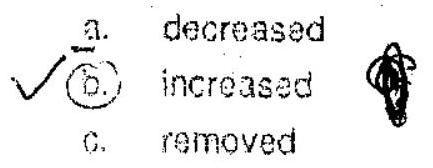
\includegraphics[max width=\textwidth]{2022_11_11_ca6a6c1a0324ee23e523g-02(1)}

\begin{enumerate}
  \setcounter{enumi}{6}
  \item Cabiumoxide is also called Cao
  \item 3lakedime.\\
(b.) quicklime.\\
c. hydratedlime.\\
d. denydrated lime.
\end{enumerate}

b. If a wator tank is filled with water to a height of $40 \mathrm{it}$ and the tank is 20 it in diameter, the pressure at the base of the tant is psi.

$$
\begin{array}{ll}
\text { a. } & 17.32 \\
\text { b. } & 62.4 \\
\text { o. } & 144 \\
\text { d. } & 1440
\end{array}
$$

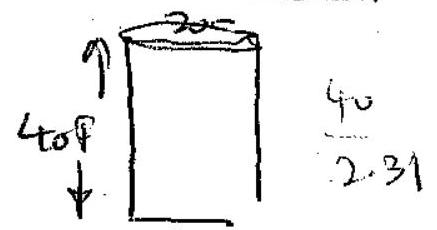
\includegraphics[max width=\textwidth]{2022_11_11_ca6a6c1a0324ee23e523g-02(2)}

\begin{enumerate}
  \setcounter{enumi}{8}
  \item Fon a sanity standpoint, the pressure in a distribution system shouid inl bu alomed to fall to zero because\\
a. the chlorine residual will escape.\\
b. Low pressure allows bacteria to multiply.\\
c. Groundwator may enter and backsiphonage may occur.\\
d. none of the above.

  \item Which one of the rollowing is a hazard when using hydrofluosilicic acid?\\
a. corrosiveness\\
b. explosiveness\\
c. Nlammability\\
d. none of the above

  \item Slatic suction head plus friction suction head plus static discharge head plus ifction discharge head makes up the of a pump.\\
a. operating pressure\\
b. pump curve\\
c. total dynamic head\\
d. velocity head

  \item The volume of a cone with a radius of 8 it and a height of 12 it is $f^{3}$

  \item 84

  \item 256\\
c. 502\\
d. 804

\end{enumerate}

Cone doblum: $1 / 3$ of cyplinder.

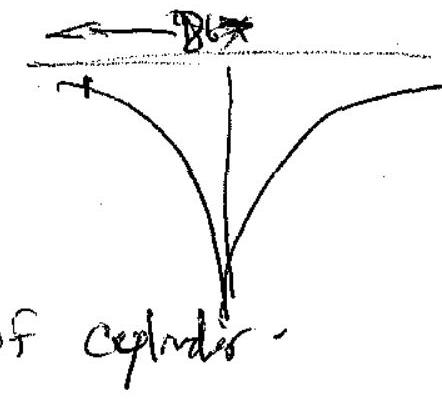
\includegraphics[max width=\textwidth]{2022_11_11_ca6a6c1a0324ee23e523g-02(3)}

\begin{enumerate}
  \setcounter{enumi}{12}
  \item Water is at its greatest density at a temperalure of
\end{enumerate}

$$
\begin{array}{ll}
\text { a. } & 32^{\circ} \mathrm{F}\left(0^{\circ} \mathrm{C}\right) . \\
\text { b. } & 39.2^{\circ} \mathrm{F}\left(4^{\circ} \mathrm{C}\right) \\
\text { c. } & 37^{\circ} \mathrm{F}\left(3^{\circ} \mathrm{C}\right) . \\
\text { d. } & 40^{\circ} \mathrm{F}\left(7^{\circ} \mathrm{C}\right) .
\end{array}
$$

\begin{enumerate}
  \setcounter{enumi}{3}
  \item A heay grom of algae in a surface inat reseryoir will havo min on\\
of he following offects on the water?
\end{enumerate}

will hate no effect on the ort

(lex) $\mathrm{CO}_{2}$

a. ounting the odor-producing organisms

b. Jiluling the sample with distill water.

a. itinithe sampewinortm wale

\begin{enumerate}
  \item natoing the ocor ayainst tha standards.\\

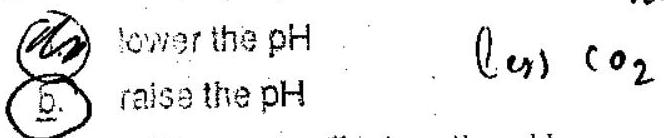
\includegraphics[max width=\textwidth]{2022_11_11_ca6a6c1a0324ee23e523g-03}\\
heary algare consumas $\mathrm{CO}_{2}$ in water.
\end{enumerate}

So pit increuse

\begin{enumerate}
  \setcounter{enumi}{11}
  \item A orntuga gunp when ocoating rondly shows a dishargo pressure
\end{enumerate}

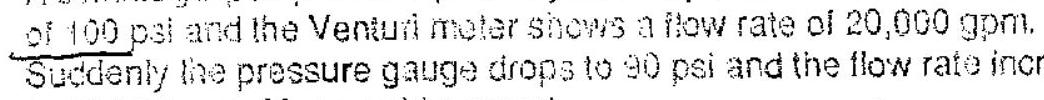
\includegraphics[max width=\textwidth]{2022_11_11_ca6a6c1a0324ee23e523g-03(1)}

1623,000 gon. You would suspect\\
3. A Julty gauge and inanomotor lubs.\\
b. Jlarge leak in the pump discharge line.\\
(c.) oreign matter caugh in the Venkuri-tube throat.\\
¿. the packing is sucking air.

\begin{enumerate}
  \setcounter{enumi}{16}
  \item A lest on a water supply showed a hardness of $232 \mathrm{mg} / \mathrm{L}$. If this is reduced by 21 percent, what should the hardness of the water be aftar lreatment?\\
a. $138 \mathrm{mg} / \mathrm{L}$\\
b. $174 \mathrm{mg} / \mathrm{h}$\\
$232 \times 0.79$\\
c. $\quad 183 \mathrm{mg} / \mathrm{h}$\\
d. $211 \mathrm{mg} / \mathrm{L}$

  \item A water lieatmont plan* used 647 chlorine cylinders during one year's operation. The average with dawalfom oach cylinder was 138 tb. What was the lolat number of pounds of chlorine used?\\
a. $\quad 89,875 \mathrm{lb}$\\
(b.) $89,286 \mathrm{lb}$\\
c. $70,872 \mathbb{1 b}$\\
d. $\quad 59,876 \mathrm{lb}$

\end{enumerate}

\section{$647 \times 138$}
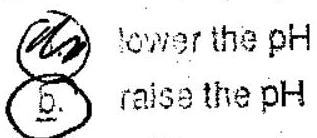
\includegraphics[max width=\textwidth]{2022_11_11_ca6a6c1a0324ee23e523g-03(2)}

\begin{enumerate}
  \setcounter{enumi}{18}
  \item The bacteriocidal action of free ayailable chlorine compared with that of combined available chlorine is
\end{enumerate}

$$
\begin{aligned}
&\text { a. greater. } \\
&\text { b. loss. } \\
&\text { c. the same under most conditions. } \\
&\text { d. nol possible to determine. }
\end{aligned}
$$

\begin{enumerate}
  \setcounter{enumi}{19}
  \item The condition in infants known as methemoglobinemia is thought to be causod mainly by high concentrations of\\
a. phosphate.\\
b. nitrate.\\
c. Fluoride.\\
d. Chloride.

  \item The flow inrough a water trestment plant is $27,777 \mathrm{gpm}$. The flow is mod.

\end{enumerate}

$$
\begin{array}{ll}
\text { a. } & 0.27 \\
0 . & 17 \\
6 & 27 \\
\text { d. } & 10 \\
\hline
\end{array}
$$

$$
27,777 / 695
$$

\begin{enumerate}
  \setcounter{enumi}{21}
  \item Vortion turine pumps that are used in wells may be oil lubricated or Maler fubricated. Operators should use extreme care not to start any Waler-lubicated pump belore making sure that the\\
a. bearings are dry.\\
(b) bearings are wet.\\
c. yalve on the discharge side is closed.\\
i. vaive on the suction side is closed.

  \item The chenical symbol for potassium is\\
a. Al.\\
b. Ba.\\
C. K.\\
d. Po.

  \item Concentrations of hardness are expressed in terms of\\
a. a percent of calcium hardness to total hardness.\\
b. calcium and magnesium hardness.\\
c. milligrams per litre as $\mathrm{CaCO}_{3}$.\\
d. Soft to very hard. 25. The amperometric titration method is usad to measure\\
a. aikalinity.\\
b. chlorine residual.\\
c. $\mathrm{oH}$\\
d. total hardness.

  \item Wak the correct number ol coliform oer $100 \mathrm{~mL}$ when a membrane filter count shovs 43 coliform colonias and $1.00 \mathrm{~mL}$ of sample was fitered.\\
a. 130\\
b. 4300\\
c. 43,000\\
d. 430,000

  \item Nonsattleaole solids are classified as solids.\\
a. suspended, colloidal, and tissolved\\
b. colloidal, dissolved, and total dissoned\\
c. colloidal, bactorial, and susponded\\
d. colrse, fine, and ary tin?

  \item Ycu pumo oroka down, your shrago lank oontained 1 mil gal, and water was being wisthorawn at a das di $0.5$ mgd, iow long would it

\end{enumerate}

take tor the tank to emply?\\
a. I day\\
b. 2 dizys\\
c. 3 days\\
d. It days

\begin{enumerate}
  \setcounter{enumi}{28}
  \item The chemical formula for copper suifate is\\
a. SaCO.\\
b. $\mathrm{CaCO}_{3}$.\\
c. $\mathrm{CuSO}_{4} \cdot 5 \mathrm{H}_{2} \mathrm{O}$\\
d. $\mathrm{H}_{2} \mathrm{SO}_{4}$.

  \item A yeniuri lube increases the velocity and decreases the pressyre as water flows tirough it. This type of woe is used to\\
a. aorate the water.\\
b. measure the amount of chlorine in the water.\\
c. Tneasure the amount of suspended solids in the water.\\
d. measure the rate of waler flowing through it.

  \item The amount ol chlorine actually used can best be deternined by\\
a. calculating the chlorine demand.\\
b. converting the dosage rate at $8 \cdot h$ intervals to pounds used.\\
c. The WAG method.\\
d. use ol scales. 32. The most hazardous condition associated with storage areas, sturry tanks, or other contined spaces where wet activated carbon is present is (a.) combustion.

\end{enumerate}

c. lires.

d. oxidation.

\begin{enumerate}
  \setcounter{enumi}{32}
  \item Two lesloused to monitor the disinfection process are
\end{enumerate}

a. chlorine dernand and cilorine residual lests.

b. Shlorine residual and bacteriological tests.

c. mombrane fitter and multiple-tube tests.

¡. Standard plate count and chitorine demand test.

\begin{enumerate}
  \setcounter{enumi}{33}
  \item A calm area within a settling basin necessary for suspended materials to sotle is the zone.
\end{enumerate}

a. inlat

b. outlet

is. sottling

d. studge

\begin{enumerate}
  \setcounter{enumi}{34}
  \item The water treatment chemical copperas is\\
a. aluminum sulfate.\\
b. chlorinated lime.\\
c. copper sulfate.

  \item iron sulfate.

  \item As long as free chlorine and organic precursors are available, the total trihalomethane (TTHM) production will most probably\\
a. Continue to fall.\\
b. continue to rise.\\
c. Fall and then rise.\\
d. Stay the same.

  \item The iree chlorine residual in water is measured as the amount of\\
a. chloride in water.\\
b. chlorine applied as measured in milligrams per litre.\\
c. chlorine in raw water as comes from the stream, reservoir, or well.\\
d. Uncombined chlorine that remains in the water after the chlorine has been applied and allowed to react. 33. Chtorine use at a water treatment plant averages $81 \mathrm{~b} / \mathrm{d}$. Assuming that the avorage daily flow is $13 \mathrm{rrgd}$, the dosage rate is $\mathrm{mgg} / \mathrm{L}$.\\
a. $0.5$\\
b. $0.75$\\
c. $1.0$\\
d. 715

\end{enumerate}

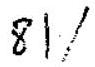
\includegraphics[max width=\textwidth]{2022_11_11_ca6a6c1a0324ee23e523g-07}

\begin{enumerate}
  \setcounter{enumi}{38}
  \item Tha chenital formula for caichm carbonate is\\
a. $\mathrm{C} 3 \mathrm{CO}_{3}$.\\
b. $\quad \operatorname{CuSO} 4$.\\
c. $\mathrm{NaCl}$.\\
d. NaCo.

  \item The chemical formula for alum is\\
a. ALsO.\\
b. AlC $\mathrm{ACO})$

  \item $1 / 2013 \cdot 111100$\\
d. Fe(304)

  \item I' yabe in pipeine is dosed too rapldy it will cause the waler in that pipaline to cone to a suddon siop, sausing waves of high pressure tha: oscillo back and forth in tho pipaline. This reaction is commonly krown as\\
a. hydraulic gradient.\\
b. pipeline dynamics.\\
c. static oscillation.\\
d. Water haminer.

  \item Eight coxss of packing (tor pumps) were delivered, and the invoice shomed $\$ 15.93$ each. What is the total cost of packing?\\
a. $\$ 106.34$\\
b. $\$ 109.31$\\
c. $\$ 111.51$\\
$\$ \times 13 \cdot 43$\\
d. $\$ 127.44$

  \item A cylindrical tank with a [adius of 5 it is filled to a depth of 10 it with water. Appro;imalely how many gallons of waler does it contain?\\
a. $578 \mathrm{gal}$\\
b. $785 \mathrm{gal}$\\
c. $870 \mathrm{gal}$\\
$10 \times 10 \times 0.785 \times 10 \times 7.49$\\
d. $\quad 3870 \mathrm{~g}$ gal 44. One of the most common causes of errors in water quality analysis is\\
a. contaminatedreagents.

  \item improper sampling.\\
c. poor laboratory equipment.\\
i. pcorly trained analysts.

\end{enumerate}

as. Ond of the problems with ductile-iron pipe is\\
(i.) curting the pipe.\\
b. pipe llexibility.\\
c. lack of being malleable.). to hummar.\\
d. limitation on piessure.

\begin{enumerate}
  \setcounter{enumi}{39}
  \item A cylindrical tank with a radius of 5 t and a height of 10 ft is filled with Malar. If 3 tb of a chemical is dissolved in the water. what is the dosage?\\
a. $112 \mathrm{mg} / \mathrm{L}$\\
D. $75 \mathrm{mg} / \mathrm{L}$\\
S. $31 \mathrm{mg} /$\\
$3 \frac{187.18}{1.0000} \times 8.3 \%$\\
d. $27 \mathrm{mg} i \mathrm{~L}$

  \item Oonfitual pump noises will mosi ihkely be due to

\end{enumerate}

$$
\begin{aligned}
&\text { a. cavitation. } \\
&\text { b. excessive head pressure. } \\
&\text { 6. high velocity. } \\
&\text { d. sand. }
\end{aligned}
$$

\begin{enumerate}
  \setcounter{enumi}{42}
  \item To tacilitate check-valve ropairs, a gate valve should be placed\\
a. beiween the pump and the check valve.\\
b. in paraliel to the check valve.\\
c. On the discharge side of the check valve.\\
d. on the suction side of the pump.

  \item The invart elevation of a pipe relers to the elevation of the center\\
a. line of the pipe.\\
b. of the bottom on the inside.\\
c. of the bottom on the outside.\\
d. of the top on the inside.

  \item The term "clarification" is most closely related to\\
a. all in-plant treatment processes.\\
b. purification.\\
c. sedimentation.\\
d. the coagulation and flocculation processes. 51. Five grains per gallon is\\
a. 35\\
b. 53\\
$5 \times 77$

\end{enumerate}

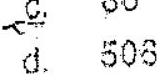
\includegraphics[max width=\textwidth]{2022_11_11_ca6a6c1a0324ee23e523g-09}

\begin{enumerate}
  \setcounter{enumi}{51}
  \item Wydrogen sulfide in well water will cause ho water to have an ocor similar to\\
a. ammonia.\\
b. chlorinegas.\\
\& rottan eggs.\\
d. lisheggs.

  \item Which lacoratory lest in a water plant is concerned with indicator changes at $\mathrm{pit} 8.3$ and about $\mathrm{pH} 4.5$ ?\\
(a.) total hardness\\
b. total chlorine residua!

  \item $\mathrm{oH}$\\
(a) akalinity $V$

  \item Which on of the toliowng typos of purga works on the basis of mertia or mass mokeg in a circulat motion?\\
a. air lith\\
(0.) canifíugal\\
c. diaphragm\\
d. gear

  \item The purpose of the jar test is to determine the\\
a. amount of chlorine 10 add for breakpoint chlorination.\\
b. correct amount of coagulant lo use for proper coagulation.\\
c. langth of the llash mix.\\
d. Proper amount of mixing and settling time to remove turbidity.

  \item The indicator methyl orange is used in the test for\\
a. akalinity.\\
b. chlonine residus.\\
c. pH.\\
d. total hardness.

  \item Hardness in water is caused mainiy by the presence of\\
a. Calcium and magnesium compounds.\\
b. iron and manganese compounds.\\
c. lime and soda ash.\\
d. turbidity and suspended solids. 5a. Wator that is high in sulfate can cause

\end{enumerate}

$$
\begin{aligned}
&\text { a. diarmea. } \\
&\text { b. hardening of the arteries. } \\
&\text { c. motting of tooth enamel. } \\
&\text { d. Staining of plumbing fixtures. }
\end{aligned}
$$

\begin{enumerate}
  \setcounter{enumi}{58}
  \item The aituent wiir of a clarifler is located along the rim of a 60 it diameter lank. The langth of the weir is it.
\end{enumerate}

$$
\begin{array}{ll}
\text { a. } & 188 \\
\text { b. } & 201 \\
\text { c. } & 248 \\
\text { d. } & 300
\end{array}
$$

Q0. A number of grab sample test results that are averaged together conotitute\\
2. acompositu test result.\\
b. a poor analytical procedure.\\
Q. an average conceniration.

\begin{enumerate}
  \item Grounds for viokting state or tederal regulations.

  \item The sorm aeration is detined as bringing water into intimate contact with

\end{enumerate}

$$
\begin{aligned}
&\text { 3. air. } \\
&\text { b. carbon dioxide. } \\
&\text { c. nydiogen sulfide. } \\
&\text { d. methane. }
\end{aligned}
$$

\begin{enumerate}
  \setcounter{enumi}{61}
  \item Which of the following types of pumps works on the principle of a decrease in the overall specific weight of a confined column of a gaswater mixture?
\end{enumerate}

$$
\begin{aligned}
&\text { a. air ift } \\
&\text { b. centrifugat } \\
&\text { c. diaphragm } \\
&\text { d. piston }
\end{aligned}
$$

\begin{enumerate}
  \setcounter{enumi}{62}
  \item A lank holding $2340 \mathrm{gal}$ fills in $12 \mathrm{~min}$. The rate of flow is gpm.\\
a. 195\\
b. 234\\
c. 284\\
d. 382 64. The chlorine room should be constructed so it can be entered only from tha\\
a insido of the buiding.\\
b. Noratory.\\
c. ouside and inside of the butiding.\\
g. cutide of the ouiding.\\

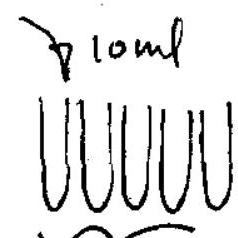
\includegraphics[max width=\textwidth]{2022_11_11_ca6a6c1a0324ee23e523g-11}
\end{enumerate}

$5+\tan n$


\includegraphics[max width=\textwidth]{2022_11_11_ca6a6c1a0324ee23e523g-11(1)}

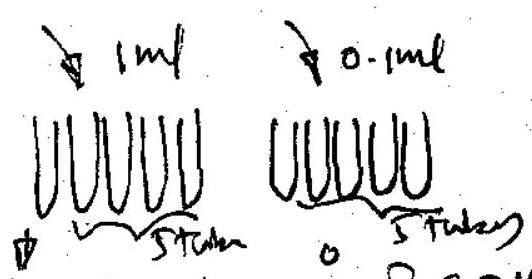
\includegraphics[max width=\textwidth]{2022_11_11_ca6a6c1a0324ee23e523g-11(2)}

Thiubate at 350 fur 24 hon

\begin{enumerate}
  \setcounter{enumi}{64}
  \item A rectangular ground slorage tank is no-fi wide, 120-it long, and 12-it deap. The tank holds gal.\\
a. $8 \hat{0}, 400$\\
b. $0+6,272$\\
c. 720,576\\
d. $\quad 500,000$
\end{enumerate}

$60 \times 120 \times 12 \times 7.48$

\begin{enumerate}
  \setcounter{enumi}{65}
  \item Dastyinon st harmfut oacinia oy chornd is disectly related to\\
a. Contet time and ohorine curcentation.

  \item Jtician chlorine cosacgolevels.\\
i. Wether or not bradgoint ondmation is practiced.\\
d. Whether prechorination is practiced.

  \item What type of treatmens should be given whon a well produces red water?\\
a. huoride removal\\
b. taste and odor control\\
c. Bedimentation\\
d. pHadjustment, aeration, and filtration

  \item The chernical that is most commonly added to reservoirs for the control of gigan is\\
a. aluminum sulfate.\\
b. calcium hypochlorite.\\
c. copper sulfale.\\
d. sodium chloride.

\end{enumerate}


\includegraphics[max width=\textwidth]{2022_11_11_ca6a6c1a0324ee23e523g-11(3)}

\begin{enumerate}
  \setcounter{enumi}{68}
  \item The slandard sample for the multiple-fube fermentation method of testing for colionm bacteria consists of portions.
\end{enumerate}

a. $\operatorname{ten} 5-\mathrm{mL}$

b. 1 in 10-ml.

(c) five 10-mL

\begin{enumerate}
  \setcounter{enumi}{2}
  \item $\operatorname{len} 10-m k$ 70. Recent studies onprechlorination practices point out that the interaction of chiorine with organic matter in raw water forms\\
a. carcinogens.\\
b. Iysergic acid.\\
c. other odor-related compounds.\\
d. irinalomethanes.

  \item Anew water traatment facility for a small town is estimated to cost $\$ 1,493,472$. What is the avarage cost per person if 1980 people live in the bo'nn?

\end{enumerate}

$$
\begin{array}{ll}
\text { d. } & \$ 5720 \\
\text { b. } & \$ 2750 \\
\text { c. } & \$ 752 \\
\text { d. } & \$ 572
\end{array}
$$

\begin{enumerate}
  \setcounter{enumi}{71}
  \item The purpose in practicing breakpoint chlorination is to

  \item elirminat laste and odor.\\
b. Increass the contact time needed to kill disease-causing organisms.\\
c. produce a free chlorine residual, which is an elfective disinfectant\\
d. reduce chlorine demand.

  \item Bacterial pollution moving underground in shattered limestone\\
a. will be removed in $10 \mathrm{if}$.\\
b. will be removed in $100 \mathrm{ft}$.\\
c. will be removed in less than $1 \mathrm{mi}$.\\
d. may never be removed.

  \item How many milligrams per litre of chlorine will be added when $10 \mathrm{lb}$ of chlorine gas is added to 333,000 gal of water?\\
a. $8.34 \mathrm{mg} / \mathrm{L}$\\
b. $4.17 \mathrm{mg} / \mathrm{L}$\\
c. $3.6 \mathrm{mg} / \mathrm{h}$\\
d. $\quad 0.5 \mathrm{mg} / \mathrm{h}$

  \item The totai dynamic head against which a pump must operate\\
a. is the friction head.\\
b. is the static head.\\
c. is the sum of the static head and the head due to friction loss. d. must always be above the shutoff head. 76. A centrifugal-type pump should never be nun empty except momentarily because\\
a. a sarious counterpressure would be buit up by excessive vacutm.

  \item it is useless to run a pump without geiting water.\\
c. He excessive end thrust or the shat would damage the thrust byating.\\
d. Iho parts lubricaied by water would be damaged.

  \item When a centrifugal pump with new packing is started and the packing seoms to leak air, the proper procedure is to\\
a. stop the motor and repack the stuifing box.\\
b. put in some havy oil and then gradually tighten the gland.\\
c. Dut in more packing.\\
d. Ignore the condition.

  \item Cotrmum coagulant dosage can be ostachish by\\
a. obsenving the pilot ither.

  \item periorming jar bests.

  \item Cororning total solic lests.\\
¿. Tho breakpoint of chlornation.

  \item Which word best describes "ha chemical combination of substances in solution so as to cause separation in the insoluble form"?\\
a. stabilization\\
b. saturation\\
c. precipitation\\
d. coagulation

  \item If the llow through a water treatment plant is $300,000 \mathrm{gpd}$ and a dosage of $2 \mathrm{mg} /$ of chemical is applied, how many pounds of chemical will be used in 30 days?\\
a. $\quad 100 \mathrm{~b}$\\
D. $150 \mathrm{lb}$\\
c. $175 \mathrm{~b}$\\
d. $200 \mathrm{bb}$

  \item Corrosiye waters can be the result of the presence of\\
a. acids,\\
b. calcium.\\
c. magnesium.\\
d. organic material. g2. A subslance added to water to promote the formation of a protective film in transmission pipes is known as\\
a. a pacitier.\\
b. a passivator.\\
c. an inhibitor.\\
ci. Cathodic protection.

  \item How mainy pounds of a chemical must be added to $50,000 \mathrm{gal}$ of water 10 produce a dosage of $75 \mathrm{mg} / \mathrm{L}$ ?\\
a. $15 \mathrm{lb}$\\
b. 3116\\
c. $60 \mathrm{lb}$\\
c. $150 \mathrm{ib}$

  \item Tho volume of water contained in a storage tank 14 ft in diameter and 20-ft desp is approximately $\mathrm{Ht}^{3}$\\
a. 900\\
b. 2000\\
$\Xi \quad 3100$\\
d. 4200

  \item Bluestone is a\\
a. common name for copper sulfate.\\
b. mineral in water that causes blue stains.\\
c. mineral not dissolvable in water.\\
d. stone for sharpening chisels.

  \item The outlet of a forced yentilation system for a chlorinator room should be located\\
a. above the window.\\
b. near the floor.\\
c. on the roof.\\
d. 6 ft above the floor.

\end{enumerate}

B7. Water leaking to the suriace after operating an old valve probably is caused by\\
a. a broken stem.\\
b. dried out packing.\\
c. plugged weep holes.\\
d. none of the above. 83. Pathogens are best described as\\
a. an acute case of indigestion.\\
b. an indicator test for viruses.\\
c. cancer-producing agents.\\
d. disease-causing organisms.

\begin{enumerate}
  \setcounter{enumi}{88}
  \item How a'e values checked to determine that they are holding properly?\\
a. by compressed air\\
b. by electrostatic test\\
c. by a pressure test\\
d. by a torque wrench

  \item Activated carbon is used to reduce\\
a. alkalinity,\\
b. nardness.\\
c. pit.\\
d. tastes and odors.

  \item Huy many gallons does 1000 it of 15 -in-dametat pipe contain?\\
a. 04 gal\\
b. $1227 \mathrm{gal}$\\
c. $2295 \mathrm{gal}$\\
$15 \times 15 \times 0=0408 \times 1000$\\
d. $9179 \mathrm{gal}$

  \item When hard water is softened by the zeolite ion-exchange process, which substance is exchanged for calcium and magnesium and will appear in the product water?\\
a. chloride\\
b. nitrate\\
c. sodium\\
d. Suliate

  \item A chemical commonly used for coagulation in water ireatment is\\
a. alum.\\
b. chtorine.\\
c. copper sulfate.\\
d. soda ash.

  \item The disintection process kills\\
a. all bacteria.\\
b. onlyprotozoans.\\
c. pathogenic bacteria.\\
d. all algae.

\end{enumerate}

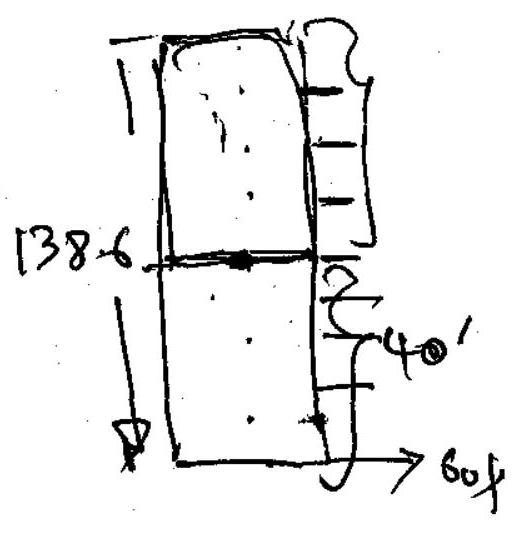
\includegraphics[max width=\textwidth]{2022_11_11_ca6a6c1a0324ee23e523g-16}

\begin{enumerate}
  \setcounter{enumi}{34}
  \item By continuously withdrawing chlorine, how many pounds per day can be ivithdrawn salely from a 150 -lb cylinder at room temperature without the line rreezing?\\
a. $10 \mathrm{lb} / \mathrm{d}$\\
Q. $40 \mathrm{l} 3 / \mathrm{d}$\\
c. $70 \mathrm{lb} / \mathrm{d}$\\
d. $100 \mathrm{~b} / \mathrm{d}$

  \item A rectangular lank measures $80-1 \mathrm{t}$ long, 30 -ft wide, and 20 -ft deep. If $100,000 \mathrm{gal}$ of water is pumped into the tank, how high will the level of the tark rise?\\
a. $2.5 \mathrm{ft}$\\
b. $5.6 \mathrm{ft}$ $10, ; 00$\\
c. $25.5 \mathrm{ft}$\\
d. $55.5$ t?

  \item What is the amount of chlorine required to treat $5 \mathrm{mgd}$ to provide a $0.8-\mathrm{mg} \mathrm{L} 0$ sidual and satisiy $2.4-\mathrm{mg} / \mathrm{L}$ chlorine dernand?\\
a. $33.33: \mathrm{ib}$\\
b. $\quad 66.67 \mathrm{lb}$\\
$3 \cdot 2$\\
c. $100,001 b$\\
d. $\quad 133,33 \mathrm{~b}$

  \item What is the detention time in a storage tank $20-\mathrm{ft}$ high and $30 \mathrm{ft}$ in diametar, when the rate of flow is $500,000 \mathrm{gpd}$ ?\\
a. $2 n 10 \mathrm{~min}$\\
b. $3 \mathrm{~h} 48 \mathrm{~min}$\\
c. $4 \mathrm{~h} 27 \mathrm{~min}$\\
d. $5 \mathrm{~h} 4 \mathrm{~min}$

\end{enumerate}

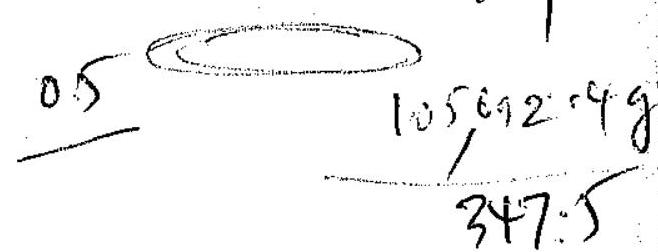
\includegraphics[max width=\textwidth]{2022_11_11_ca6a6c1a0324ee23e523g-16(1)}

\begin{enumerate}
  \setcounter{enumi}{98}
  \item If pressure at the water main is 60 psi, what is the static pressure on the plumbing faucet 40 -ft above the main?\\
a. $40 \mathrm{psi}$\\
b. $42.7 \mathrm{psi}$\\
c. $\quad 62.7 \mathrm{psi}$\\
d. $\quad 97.3$ psi\\

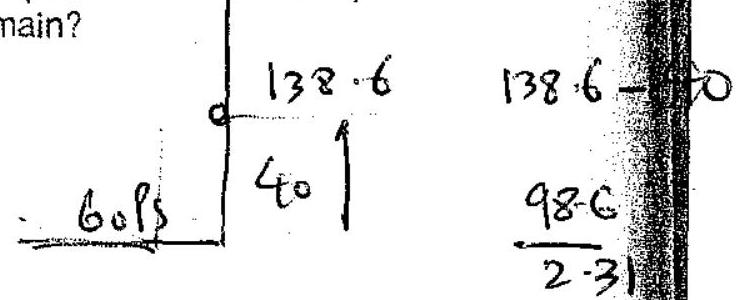
\includegraphics[max width=\textwidth]{2022_11_11_ca6a6c1a0324ee23e523g-16(2)}

  \item Discharge valves on ton containers should be positioned\\
a. according to the green arrows painted on the end of the containers.\\
b. horizontally opposite the other.\\
c. one above the other.\\
d. randomly, to simplify connection procedures.

\end{enumerate}

\section{$10 / 21 / 19$}
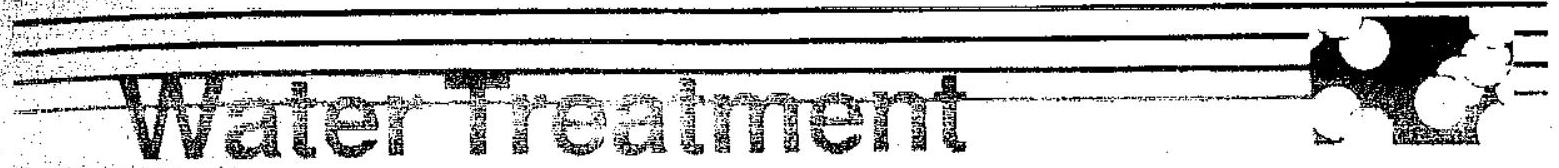
\includegraphics[max width=\textwidth]{2022_11_11_ca6a6c1a0324ee23e523g-17} ClassI\}

\begin{enumerate}
  \item When collecting a distribution-system sample for bacteriological testing, the person collecting the sample should allow the water to run before tilting the sample bottle.
\end{enumerate}

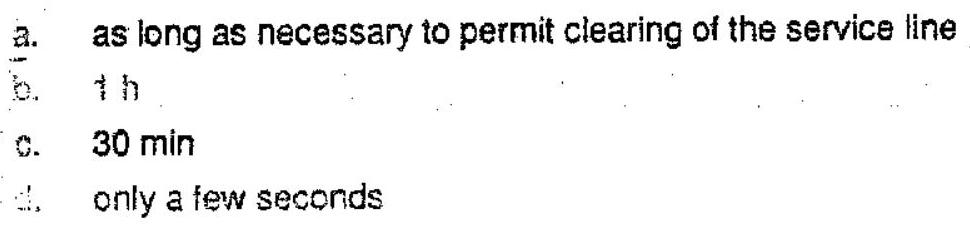
\includegraphics[max width=\textwidth]{2022_11_11_ca6a6c1a0324ee23e523g-17(1)}

\begin{enumerate}
  \setcounter{enumi}{1}
  \item The wolume of a cylinder with a radius of $5 \mathrm{ft}$ and a height of $8 \mathrm{ft}$ is $\mathrm{ft}^{3}$.
  \item 251 $10 \times 10 \times 0.785 \times 8$\\
b. 328\\
c. 451
  \item 628
\end{enumerate}

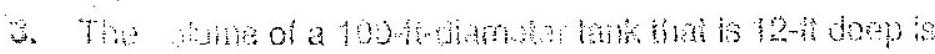
\includegraphics[max width=\textwidth]{2022_11_11_ca6a6c1a0324ee23e523g-17(2)}

$$
\begin{array}{ll}
\text { a. } & 34,200 \\
\text { 4. } & 98,500 \\
\therefore & 103.300 \\
d . & 285,200
\end{array} \quad 100 \times 150 \times 0.785 \times 12
$$

\begin{enumerate}
  \setcounter{enumi}{3}
  \item A chancal commony Leed io raise pht is\\
a. alum.

  \item calgon.\\
Q. chtorine.\\
d. lime.

  \item Raack stains on plumbing lixiures migh be attributable to\\
a. calcium.\\
b. copper.\\
c. magnesium.\\
d. nianganese. 6. One kilogram equais grams.\\
a. 10\\
b. 100\\
c. 1000\\
d. 10,000

  \item The incicator omanomatsed do dermine contarmation of drinking Waki \\
a. colitiorm group.\\
b. Giardia lamblia.\\
un as a


  \item The packing around the shaft of a centrifugal pump should be\\
a. in good condition indefinitely.\\
b. kept as tight as possible.\\
c. replaced once a month.\\
d. lightened just enough to allow an occasional drop of liquid to escape.

  \item The chemical symbol for iron is\\
a. Al.\\
b. Ca.\\
c. Fe.\\
d. Ir.

  \item One pound per aruare inch of prossura will raise water.\\
$2 \quad 20$\\
b. $10.5$\\
c. $62.5$\\
d. 1728

  \item Siatic head is deyinad as the

\end{enumerate}

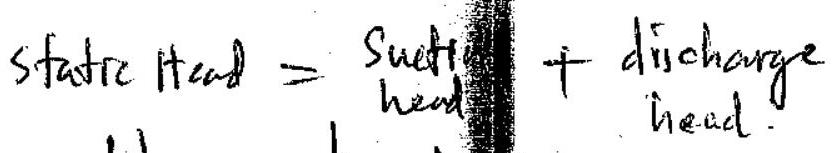
\includegraphics[max width=\textwidth]{2022_11_11_ca6a6c1a0324ee23e523g-18}

$$
H_{s}=h_{s}+\|_{d}
$$

a. energy of motion of the water.\\
b. pressure die to deoth or elevation of the water.\\
c. cressure bos the line due to irction.

\begin{enumerate}
  \item ailderoove.

  \item What is the volume of a seltling tank 100 -ft long, 25 -ft wide, and 8-ft doep?\\
a. $16,000 \mathrm{it}^{3}$\\
b. $20,000 \mathrm{it}^{3}$\\
c. $25,000 \mathrm{n}^{3}$\\
d. $36,200 \mathrm{tt}^{3}$ What is used to detect chlorine leaks?\\
a. Iy parout solilon of alunthem sulfata\\
b. 10 percent solution of ammonia hydroxide\\
c. 10 percent solution of calcium hydroxide\\
d. 10 percent solution of sodium hydroxide

\end{enumerate}

The promneraneranding the nos in tank fillod to denthot it is \$si.\\
a. 144\\
b. $52.4$\\
-. 1.\\
0. 121

The multiple-tube fermentation iest consists of three distinct tests. These tests, in the order performed, are the\\
a. preliminary, confirmed, and completed tests.\\
b. preliminary, presumptive, and confirmed tests.\\
(c.) presumptive, contirmed, and completed tests.\\
d. presumptive, preliminary, and completed tests.

Chlorine gas is\\
a. the same weight by yolume as air.\\
b. lighter than air.\\
c. lighter than air only when under pressure.\\
d. denser than air.

Polyphosonatos may bo used malm thmen to relard comonn and cirlioin soale.\\
a. ilust pit.\\
(b.) calcium scale.\\
c. reduce chlorine demand.\\
d. Pecuce taste and oriors.

Calcium nypochicrite is tomulated as a\\
a. coagulant.\\
b. d\\
c. L.\\
d. powier.

Chorine leaks in metal conairers tend to\\
a. become larger.\\
b. become smaller.\\
c. remain the same size.\\
d. seal themselves. 20. Determining the pH of water is one of the important tests of water quality. The pesuls of the whtest indicate the\\
a. chlorine residual.\\
Q. Hydrogen ion activity.\\
c. prasence of colitorm organisms.\\
d. presence of iron.


\includegraphics[max width=\textwidth]{2022_11_11_ca6a6c1a0324ee23e523g-20}\\
a. none.\\
b. one drop per second.

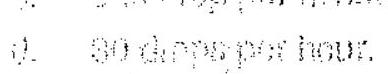
\includegraphics[max width=\textwidth]{2022_11_11_ca6a6c1a0324ee23e523g-20(1)}

\begin{enumerate}
  \setcounter{enumi}{21}
  \item A chlorine cylinder valve is thought to be leaking. If ammonia vapor is passed near the valye, the presence of a leak would be indicated by\\
a. a loud noise.\\
b. red vapor.\\
c. a rotien egg odor.\\
d. white smoke.

  \item If a fire hydrant requires a nozzle pressure of 100 psi, what head of water must be used to supply it?\\
a. $231 \mathrm{ft}$\\
b. $63.3 \hat{i t}$\\
c. $32.1 \mathrm{ft}$\\
d. 21 it

\end{enumerate}


\includegraphics[max width=\textwidth]{2022_11_11_ca6a6c1a0324ee23e523g-20(2)}\\
a. Wen the pipe is in the storage yard.\\
b. aftor the pipe is delivered to the job site.\\
c. aties the pipe is laid in place.\\
d. al the manufacturer's plant.
%
%\begin{enumerate}
%  \setcounter{enumi}{24}
%  \item Caroon chicide in mater will\\
%a. ciecrease tubicity.\\
%b. Incieaso urbicity.\\
%C. juarth.\ذ. 

\begin{itemize}
    \item A pneumalic jiector lits water from low points to higher levels, The devica yed to achiove this is a(m)\\
(a.) air compressor.\\
b. axial-flow pump.\\
c. centrifugal pump.\\
id. plunger-iype pump. 27. Pressure is commonly measured in\\
a. British themalunits.\\
b. million gallons per day.\\
c. milligrams per litre.\\
d. pounds per square inch.
 Mechanical seals are being installed in pumps because\\
(i.) ding mind indelede that sal alminte.\\
b. Seals prevent cross connections with potable water.\\
c. seals will take more shatt misalignment than packing.

  \item hom is then hom ound tyailable on the market.

\end{itemize}


\includegraphics[max width=\textwidth]{2022_11_11_ca6a6c1a0324ee23e523g-21}\\
a new ohiorine cylindor?\\
a. air and water regulator\\
b. fiber washer\\
c. needle valve and seat\\
d. pressure regulator

\begin{enumerate}
  \setcounter{enumi}{29}
  \item A major cause of pump and motor shatt coupling wear is a\\
a. discharge pressure too high.\\
b. low suction pressure.\\
c. misalignment between pumps and motor flanges.\\
d. worn-out seal.

  \item Filters in a water treatment process are primarily for removing or reducing\\
a. calcium and magnesiumsuliates. - ion exchange\\
(c) tastes and osors - Frituation\\
(d.) turbidity - Coaguation \& flocibato

  \item A watid toatment plan recayes an dyerage low of $261 \mathrm{gpm}$. What is the dainy tora flow to the plent?\\
a. $\quad 0.32 \mathrm{mgd}$\\
(1.) $0.38 \mathrm{mgc}$\\
c. $\quad 0.48 \mathrm{mgd}$\\
d. $\quad 1,4 \mathrm{mgc}$

  \item The froe chlorine residya in walot is int amount of\\
a. chlorine applied as measured in milligrams per litre.\\
o. chlorine in raw wator as is comes from the stream, reseryoir, or well.\\
c. chlorides in the water.\\
d. Uncombined chlorine that remains in the water atter the chlorine has teen oppliad and allowed to react.

\end{enumerate}

\section{CERTFICATOO STUDY GUIDE}
\begin{enumerate}
  \setcounter{enumi}{33}
  \item The chemical name for muriatic acid is
\end{enumerate}


\includegraphics[max width=\textwidth]{2022_11_11_ca6a6c1a0324ee23e523g-22}\\
b. phosphoric acid.\\
c. hydrochioric acid. 10\% HC\\
c. carbonic acid.

\begin{enumerate}
  \setcounter{enumi}{34}
  \item A chonisa noidual m salet can be determined by using the reagent\\
a. diethyi-p-phenylenediamine (DPD).\\
b. sthylanediaminetetraacetic acid (EDTA).
\end{enumerate}

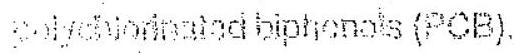
\includegraphics[max width=\textwidth]{2022_11_11_ca6a6c1a0324ee23e523g-22(1)}


\includegraphics[max width=\textwidth]{2022_11_11_ca6a6c1a0324ee23e523g-22(2)}

\begin{enumerate}
  \setcounter{enumi}{35}
  \item The most important use of chlorine in water treatment is as a(n)\\
a. aid to coagulation.\\
b. Algicide.\\
c. disinfectant.\\
d. oxidant for iron and manganese.

  \item What is the approximate volume in gallons occupied by $15,000 \mathrm{ft}^{3}$ of water?\\
a. $22,100 \mathrm{gal}$\\
b. $112,200 \mathrm{gal}$\\
$15,100 \times 7.48$\\
(.) $120,000 \mathrm{~m} l$\\
d. $10,00 \mathrm{dal}$

  \item The difisgrance beiween the amount of chlorine added to water and the amount of posiculal chlorine Femaining at the end of a specified contact Fariod is

  \item the cosage.\\
b. Iree ayailable chlorine.\\
c. oilorine residual.\\
d. Anterine demand.

  \item Water hat requires a large amount of soap to produce an acceptable lather is tenned\\
a. corrosive.\\
b. hard.\\
c. soit.\\
d. turbid. 40. A pump may be damaged if it is started with the discharge valve closed, if the pump is a(n)

  \item ubinsi,io?\\
b. positive-displacement pump.\\
c. centrifugal pump.\\
d. axial-low pump.

  \item Prepded water sampla bohes had tor colsoing samples ror bacteriological examination contain sodium thiosulfate crystals. It is important not to rinse out the sample tottle because the sodium thiosulfate

\end{enumerate}

$$
\begin{aligned}
& \text { a } \text { firmannan } \\
& \text { c. kills any pathogens hal hay se present in ine sample. } \\
& \text { d. neutralizes any chiorine present in the sample. }
\end{aligned}
$$

\begin{enumerate}
  \setcounter{enumi}{41}
  \item Velocity of flow in water mains is usually expressed in terms of\\
a. feet per second.\\
b. gallons per minule.\\
c. litres perioot.\\
d. milligrams per litre.

  \item A pH reading of $6.0$ in raw water indicates the sample is

  \item acid.\\
b. alkaline.\\
b. besin\\
d. neutral.

  \item The temperabue ci watet $n$ a $t$ tram is $10^{\circ} \mathrm{C}$. What is the equivalent

\end{enumerate}

$$
\begin{aligned}
& \text { 'andecature in degres - jnomeit? } \\
& \text { 3. } 82^{\circ} F \text {. } \\
& (10+40) 1.8 \quad \ldots . \\
& \text { b. } 50^{2} ; \text {. } \\
& \text { C. } 50 \% \\
& \text { d. } 42^{2}=
\end{aligned}
$$

\begin{enumerate}
  \setcounter{enumi}{44}
  \item Agrab samplo ienreserio\\
a. the quality of the water a the time the sample was taken.\\
o. approximately 21 oi water.\\
c. a time-proportional sample.\\
d. allowipopotionalsampla.
\end{enumerate}

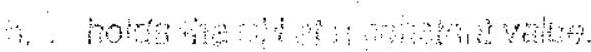
\includegraphics[max width=\textwidth]{2022_11_11_ca6a6c1a0324ee23e523g-23}

\section{CERTFICATION STUDY GUIDE}
\begin{enumerate}
  \setcounter{enumi}{45}
  \item The pH scale runs trom\\
a. $0-14$\\
b. $0-7$\\
c. 7-14.\\
d. $1-15$.

  \item Five gallons of water weigh lb.

  \item 
\end{enumerate}

b. $37.5$\\
$5 \times 8.34$\\
c. $41.7$\\
d. 394

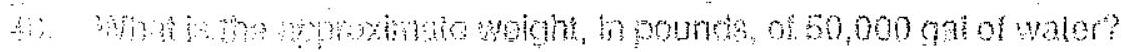
\includegraphics[max width=\textwidth]{2022_11_11_ca6a6c1a0324ee23e523g-24}\\
a. $41,000 \mathrm{lb}$.\\
b. $71,000 \mathrm{~b}$.\\
c. $170,000 \mathrm{lb}$.\\
$58,000 \times 8.34$\\
d. $417,000 \mathrm{lb}$.

\begin{enumerate}
  \setcounter{enumi}{48}
  \item The flow is $35,000 \mathrm{gpd}$. This is mgd.\\
a. $0.35$\\
b. $0.035$\\
c. $0.0035$\\
d. $0.00035$

  \item The most important factor affecting the useful life of piping is\\
a. The ability of the materiais used to resist internal and external corrosion.

  \item timand the pipa.\\
c. the thexibility of the pipe.\\
¿. Tes soothness of the inside of the pipe.

  \item A ph yaide af $7.0$ is considered to be\\acicic.\\
D. aikalines.\\
c. besis.\\
d. nouthi.

  \item The discharge-oressure gauge an a pump reads 15 psi. This is equivalent to it of head.\\
a. 5

  \item 10\\
c. 25\\
d. 35 53. Chlorine is very corrosive when combined with

\end{enumerate}

WATER TREATMENT CLASS I

a. alum.

b. carbon.

(d.) moisture.

Vang Composite / low ph

\begin{enumerate}
  \setcounter{enumi}{53}
  \item What is the surface area of a clarifier $40 \mathrm{ft}$ in diameter?
\end{enumerate}

a. Ae.

b. $\quad 630 \mathrm{ft}^{2}$

c. $1120 f^{2}$

-. $100 \mathrm{~s}^{2}$

d. sodium fluoride.

$40 \times 40 \times 0.785$

\begin{enumerate}
  \setcounter{enumi}{55}
  \item The purpose of a rotameter is to
\end{enumerate}

a. create a vacuum.


b. maintain a smooth fluid flow.\\
c. meter the flow of fluid.\\
d. reduce pressure.

b. maintain a smooth fluid flow. Torthatomethaue\\
c. meter the flow of fluid.\\
d. reduce pressure.

\begin{enumerate}
  \setcounter{enumi}{56}
  \item A valve that joins a customer's service to the water main is called the Frrabomesthere iss a:
\end{enumerate}

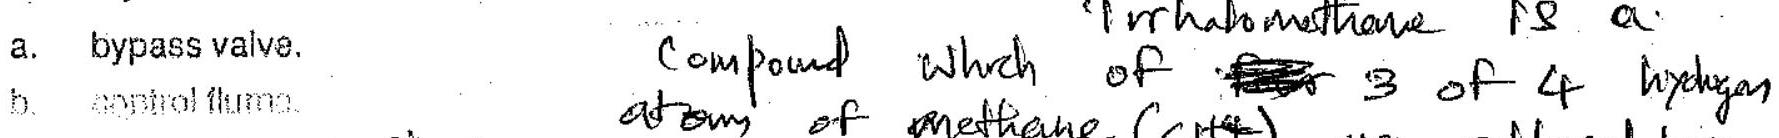
\includegraphics[max width=\textwidth]{2022_11_11_ca6a6c1a0324ee23e523g-25}

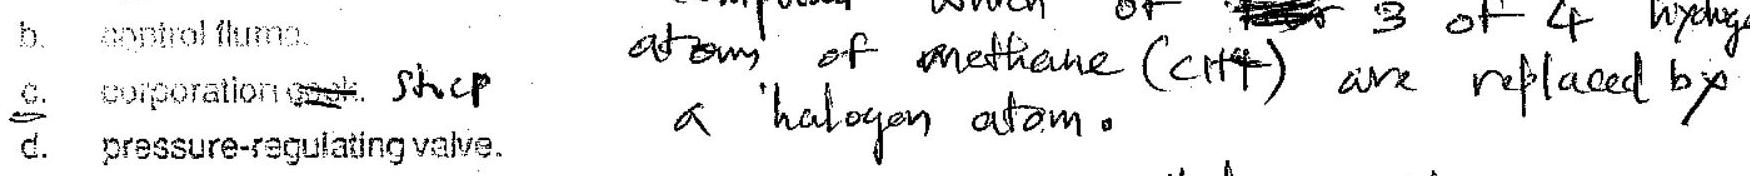
\includegraphics[max width=\textwidth]{2022_11_11_ca6a6c1a0324ee23e523g-25(1)}

EB. When compared to a 1 mil gal sesompir at the same water elevation, taken Atoms: how much pressure in he mans will a $100,000-g a l$ reservoir develop? Chlorine. Br\\
a. exactly one tenth as much pressure

b. Jess pressure

c. more pressure

$\infty$ tho same pressure

$\frac{\text { Examples of Tribal ometternas }}{\text { (i) CHF - Proflouromethane }}$

(flaroform)

5). What inlomation must co ch a naming bang attached to a switch that has been lowidod ow?

a. directions in removing 10$]$

(2) $\mathrm{ClCl}_{3}$ - Trichloromethane

b. name of nearest physician to call in case of an emergency

c. Signature of person who locked out switch and who is the only

person authorized to remove tag

d. time to unlock smith 60. Which one of the following types of meters has no moving parts?\\
a. propeller\\
i. proportional\\
c. rotameter\\
d. Venturi

\begin{enumerate}
  \setcounter{enumi}{60}
  \item The component of a centrifugal pump that is sometimes installed on the ant th wo men to hold the priming is lnown as a\\
a. casing.\\
b. drain.\\
a. 1 oothye.

  \item ff

  \item Coagulation and sedimentation alone cannot remove all of the turbidity and suspended matter in raw water. The final step in the removal of suspended matter in water is\\
a. chlorination.\\
b. filtration.\\
c. Ilocculation.\\
d. sierilization.

  \item Water weighs lb/gal.\\
a. $7.5$\\
b. $8.34$\\
c. $\quad 17.1$\\
d. $\quad 62.4$

\end{enumerate}

\begin{itemize}
  \item m. Thennon avmol or solium is
\end{itemize}

$$
\begin{array}{ll}
\text { 1. } & \text { b. } \\
\text { b. S. } \\
\text { c. Na. } \\
\text { d. K. }
\end{array}
$$

. The ouroces for fluoridating municipal water supplies is to\\
3. disintect the uater.\\
b. hatp improve the taste of the water.\\
c. help prevent dental decay.\\
d. iemove iron

 Pressura is usually measured in\\
a. cubic feet per second.\\
b. foot pounds.\\
c. gallons per minute.\\
d. pounds per square inch. 67. Chlorine valves are opened and closed with\\
a. any suitable wrench of pliers.\\
b. Gipe womh ond woudn muntet.\\
c. valve wrenches proyided with a cylinder or 1 -ton container by

\begin{itemize}
  \item the manufacturer.\\
d. Wrenches made of a special, nonsparking alloy as a safety precaution.
\end{itemize}

Q. Whiweight in aho bo of mhor?\\
a. $\quad 1.55 \mathrm{lb}$\\
b. $8.34 \mathrm{lb}$\\
c. $7.48 \mathrm{~b}$

\begin{enumerate}
  \item 3 in

  \item When opening and closing valves ni highpiossure ines, he valves should be opened\\
a. and closed as rapidly as cossible.\\
(b.) and closed slowly.\\
c. rapidly and closed slowly.\\
d. slowiy and closed rapidly.

  \item A hypochlorinator is used to fead into a watior supply.\\
(a.) hypochlorite solution\\
b. chlorine gas\\
c. chloramines\\
d. all of the above

  \item One cuoic loot of water contains gal.

\end{enumerate}

%$$
%\begin{array}{cc}
%\therefore \quad 55 \\
%\text { _. } & \quad 8.34 \\
%\text { d. } & \quad 22.4
%\end{array}
%$$

\begin{enumerate}
  \setcounter{enumi}{71}
  \item One ci the purposes of tuater storage lanks is to
\end{enumerate}

$$
\begin{aligned}
&\text { a. decrease the oxyon conteri. } \\
&\text { b. imorove the taste. } \\
&\text { o. increase the carbon dioxide content. } \\
&\text { d. supply wakr ar peek demands. }
\end{aligned}
$$

\section{Elevated water tanly to keif adeaguate pressure.}
\begin{enumerate}
  \setcounter{enumi}{72}
  \item Hed, sill, clay, and other susporded matiar in water that cause it io apoesir murky are called\\
a. cloudiness.\\
b. hardness.\\
c.. turbidity.\\
d. turbulence. 74. If the pressure gauge at the bottom of a 200 -ft standpipe reads 68 psi, what is the static head in teet?\\
a. 8614\\
b. $143 \mathrm{~A}$\\
c. $157 \mathrm{ft}$\\
d. $200 \mathrm{ft}$
\end{enumerate}

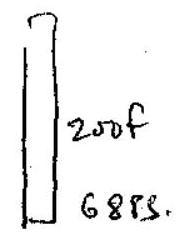
\includegraphics[max width=\textwidth]{2022_11_11_ca6a6c1a0324ee23e523g-28}

\begin{enumerate}
  \setcounter{enumi}{74}
  \item The viune of a sample shotld dependon
\end{enumerate}

(a.) what tests the sample will be used for.

b. the type of water being sampled.

ha o the ondetor.

bon many $\mathrm{s}$ mpha are neded

\begin{enumerate}
  \setcounter{enumi}{75}
  \item A cump needs new packing\\
a. if no more packing will fit into the stuffing box.\\
b. if there is any leakage from the packing gland.\\
c. when no more packing can be added.\\
(d.) When the gland follower is pulled all the way down.
\end{enumerate}

\section{Sodium hypochlorite is a}
a. compound that can be purchased in liquid solution and can be used for disinfection.

b. dry neutralizing powder for chlorine burns.

c. gas delivered in 100-16, 150-ib, and 1-ton cylinders.

\begin{enumerate}
  \item Salt that is formed when hydrochlorie acid is neutralized by uclitubytwxibe.

  \item Gas chlcrinators, when operated at a high rate of withdrawal from the cinkrina cylinder, can result in\\
a. an explosion.\\
b. ice formation on the chiorine cylinder.\\
a. ro effect.\\
d. Overheating of the gas cylinder.

  \item 1/0en a single water sample is reported as sate, this may be interpreted omean\\
a. That the water supply is adequately protected.\\
b. thal the waler supply may be regarded as safe until additional samples are requested by the city heailt officer.\\
c. That the water supply was safe at the sampling point at the time of the sampling.\\
d. none of the above. 80. In loading or untoading 150 -1b chlorine cylinders, hand trucks should be used that are equipped with\\
a. Hitamingenaty hant\\
b. a sling.\\
c. positive traction wheels.\\
d. Safety features approved by OSHA regulations.

\end{enumerate}

a1. The foos or units "pom" sppearing on a flow-rate indicator in a pumping stalusuadns\\
a. gallons perman.\\
b. gallons per man-hour.

\begin{enumerate}
  \setcounter{enumi}{81}
  \item The amount of dissolved oxygen that can remain in water depends primerily on\\
a. water temperalure.\\
b. sunight.\\
c. $\mathrm{pH}$.\\
d. other constituents.

  \item A flow of $1.55 \mathrm{it}^{3} / \mathrm{s}$ is gpm.\\
a. 150\\
b. 384 $1.35 \times 444$\\
c. 569\\
d. 696

  \item What is the chlorine domand is the residual is $0.6 \mathrm{mg} / \mathrm{L}$ and $6.6 \mathrm{mg} / \mathrm{L}$ has is a be?

\end{enumerate}

$$
\begin{aligned}
& \text { 3. } \quad 1.7 \mathrm{mg} / \mathrm{h} \\
& \text { b. } 4.0 \mathrm{mg} / \mathrm{L} \\
& \text { ¿. } \quad 3.0 \mathrm{mc} / \\
& \text { d. } \quad 7.2 \mathrm{mg} / \mathrm{h}
\end{aligned}
$$

\begin{enumerate}
  \setcounter{enumi}{34}
  \item The most edfective ph range fot iron and manganese removal is\\
a. ooliso.
  \item 
7.


\end{enumerate}

$\therefore \quad 8109$

\begin{itemize}
  \item not applinble to the constidnnts.
\end{itemize}

\begin{enumerate}
  \setcounter{enumi}{85}
  \item How many gallons per minute is a flow of $1.0 \mathrm{mgd}$ ?\\
a. $521 \mathrm{gpm}$\\
D. $681 \mathrm{gPm}$\\
c. $\quad 695 \mathrm{gpm}$\\
d. $813 \mathrm{gpm}$ 87. Disease-producing organisms are commonly called\\
?. inorganics.\\
D. microbiota.\\
c. pathogens.\\
d. protozoa.

  \item One pound per square inch pressure will support a column of water Bnt ...... it nigh\\
a. $1.55$\\
b. $2.31$\\
a. $\because 10$\\
i.

  \item Vent openings on reservoirs and clearwelis should be\\
a. chlorinated frequently.\\
b. provided with an overlapping cover.\\
c. sealed during winter.\\
d. screened.

  \item You are chlorinating a well supply and the chlorine demand jumps from $0.9 \mathrm{mg} / \mathrm{L} 103.0 \mathrm{mg} / \mathrm{L}$. This is indicative of\\
a. weak chlorine.\\
b. pollution.\\
c. more water being pumped.\\
d. all of the above.

\end{enumerate}

\begin{tabular}{llllll}
\hline
 &  & Certification Leval &  &  \\
\hline
Evaluate bacteriological characteristics of source water & $X$ & $X$ & $X$ & $X$ \\
Evaluate biological characteristics of source water & $X$ & $X$ & $X$ & $X$ \\
Evaluate chemical characteristics of source water & $X$ & $X$ & $X$ & $X$ \\
Evaluate physical characteristics of source water & $X$ & $X$ & $X$ & $X$ \\
\hline
\end{tabular}

\section{Suctertions for Stury:}
\begin{itemize}
  \item Knowiedge of nomal characteristics of water

  \item Knowledge of sanitary survey process

  \item Knowledge of watershed protection

  \item Ability to discriminate between normal and abnormal conditions

\end{itemize}

\section{Sample Questions for Class I, answers on p. 71}
\begin{enumerate}
  \item A watercourse that flows continuously at all times of the year is called\\
a. Intermittent stream\\
b. Ephemeral stream\\
c. Perennial stream\\
d. Natural stream

  \item During the night, algae causes the $\mathrm{pH}$ of the water to\\
a. Increase\\
b. Dacrease\\
c. Remain about the same as during the day\\
d. Fluctuate up or down depending on the species of algae that dominate

  \item Which of the following contributes to the creation of algae blooms?\\
a. Increased turbidity\\
b. Incressed air temperature\\
c. Increased nutrients\\
d. Increased wind action 4. Which of the following is found mainly in groundwater sources and forms a precipitate when oxidized?\\
a. Hydrogen sulfide\\
b. Methane\\
c. Radon\\
d. Iron

  \item The Riparian Doctrine is sometimes called the\\
a. Rule of Reasonable Sharing\\
b. Appropriation Doctrine\\
c. Allocation of Ground Water\\
d. Correlative Rights Rule\\

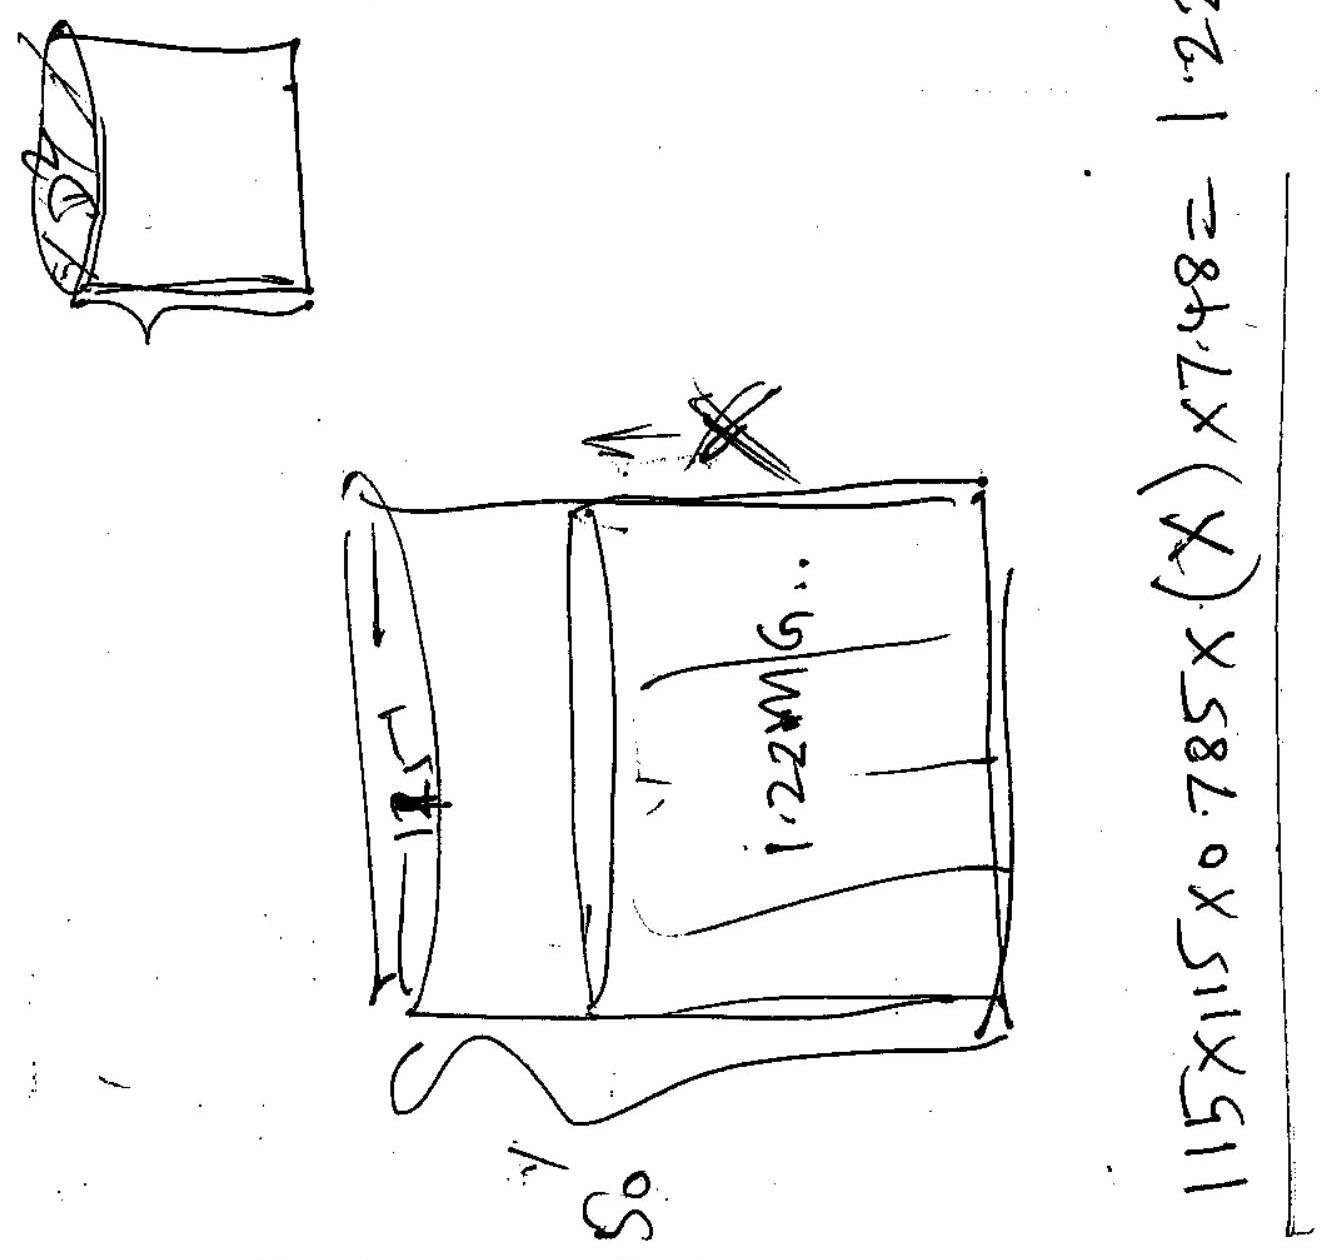
\includegraphics[max width=\textwidth]{2022_11_11_ca6a6c1a0324ee23e523g-32}

\end{enumerate}

\section{.UATE CHARACTERISTICS OF SOURCE WATER}
\section{Sample Questions for Class II, answers on p. 72}
\begin{enumerate}
  \item If a water body has a high salinity and is warm, it will generally be\\
a. High in dissolved oxygen\\
b. Low in dissolved oxygen\\
c. Supersaturated with dissolved oxygen and low in total dissolved solids\\
d. Indeterminate for dissolved oxygen and total dissolved solids
\end{enumerate}

\section{Reservoir turnover is?}
a. Related to $\mathrm{pH}$ of the water\\
b. Caused by denser water at the surface sinking toward the bottom\\
c. Caused by wind craking ice on the surface\\
d. Needed to control algae growth

\begin{enumerate}
  \setcounter{enumi}{2}
  \item What does the term surface runoff refer to?\\
a. Rainwater that soaks into the ground\\
b. Rain that returns to the atmosphere from the earth's surface\\
c. Surface water that overflows the banks of the rivers during flood stage\\
d. Water that flows into the rivers after a rainfall
\end{enumerate}

\section{Hikers, bicyclists, all-terrain vehicles, and automobiles can all of watershed land adjacent to a reservoir.}
a. Improve the appearance\\
b. Discourage access\\
c. Increase the threat of erosion\\
d. Limit recreation

What is the term for a water-bearing geologic zone composed of aterial deposited by flowing rivers?

\begin{itemize}
  \item Artesian aquifer
\end{itemize}

b. Unconfined aquifer

c. Consolidated aquifer

\section{EVALUAIE CHARACTERISTICS OF SOURCE WATER}
\section{Sample Questions for Class Ill, answers on p. 73}
\begin{enumerate}
  \item What effect will algae in a reservoir have on dissolved oxygen (DO)?
\end{enumerate}

a. Lower the DO during the day and increase the DO during the night

b. Slowly increase the DO during both the day and night

c. Increase the DO during the day and lower the DO during the night

d. Slowly decrease the DO during both the day and night

\begin{enumerate}
  \setcounter{enumi}{1}
  \item What effect does alkalinity have on the use of copper sulfate as an algicide?
\end{enumerate}

a.) Copper sulfate is more effective as alkalinity increases\\
(60) Copper sulfate is more effective as alkalinity decreases

c. Alkalinity has no effect

d. Alkalinity prevents toxicity to fish

\begin{enumerate}
  \setcounter{enumi}{2}
  \item The amount of water in a water-bearing formation depends on the\\
a. Depth of the well\\
b. Size of the pump\\
c. Porosity of the formation\\
d. Type of well casing

  \item What is the main characteristic of raw water that enables blue-green algae to grow?\\
a. Presence of copper sulfate\\
b. Low $\mathrm{pH}$\\
c. High hardness\\
d. Presence of nutrients

  \item A well screen must be installed for which of the following?\\
a. All deep wells\\
b. Only shallow wells\\
c. Consolidated materials\\
(d.) Unconsolidated materials

\end{enumerate}

\section{EVALUATE CHARACTERISTICS OF SOURCE WATER}
\section{Sample Questions for Class IV, answers on $0.74$}
\begin{enumerate}
  \item What is the recommended loading rate for copper sulfate for algae control at an alkalinity greater than $50 \mathrm{mg} / \mathrm{L}$ ?\\
a. $0.9 \mathrm{lb}$ of copper sulfate per acre of surface area\\
b. $1.9$ lb of copper sulfate per acre of surface area\\
c. $2.4$ lb of copper sulfate per acre of surface area\\
d. 5.4 lb of copper sulfate per acre of surface area

  \item What is the primary origin of coliform bacteria in water supplies?\\
a. Natural algae growth\\
b. Industrial solvents\\
c. Animal or human feces\\
d. Acid rain

  \item Which of the following best defines the term specific capacity?\\
a. Amount of water a given volume of saturated rock or sediment will yield to gravity\\
b. Amount of water a given volume of saturated rock or sediment will yield to pumping\\
c. Rate at which water would flow in an aquifer if the aquifer were an open conduit\\
d. Amount of water a well will produce for each foot of drawdown

  \item The most common type of well used for public water supply systems is a\\
a. Jetted well\\
b. Driven well\\
c. Drilled well\\
d. Bored well

  \item Copper sulfate is used for algae control. Your reservoir is $1,200 \mathrm{ft}$ long and $600 \mathrm{ft}$ wide. At an application rate of $5.5 \mathrm{lb}$ per surface acre, how much copper sulfate is required?\\
a. $221 b$\\
b. $80 \mathrm{lb}$\\
c. $91 \mathrm{lb}$\\
$\frac{1200 \times 600}{4+3560} \times 55$\\
d. $107 \mathrm{lb}$

\end{enumerate}

\section{SAFETY AND EMERGENCY PREPAREDNESS}
\section{Sample Questions for Class I, answers on $p .92$}
\begin{enumerate}
  \item Which of the following diseases is capable of being transmitted by water?\\
a. Typhoid\\
b. Measles\\
c. Encephalitis\\
d. Mumps
\end{enumerate}

$$
\begin{aligned}
&C \text { - cholera } \\
&D \text { - Dystantix } \\
&H \text { - Hepatitios } \\
&P \text { - Polro } \\
&S \text { - sulmowily }
\end{aligned}
$$

$$
\text { Criradn \& Lambla }
$$

\begin{enumerate}
  \setcounter{enumi}{1}
  \item When any piece of electrical equipment is being worked on, the circuit breaker should be\\
a. Painted when repair is complete\\
b. Videotaped for future reference\\
c. De-energized and locked out\\
d. Replaced

  \item If ammonia vapor is passed over a chlorine leak in a cylinder valve, the presence of the leak is indicated by a\\
a. Yellow cloud\\
b. White cloud\\
c. Gray cloud\\
d. Brown cloud

  \item Which of the following directly impacts the treatment of drinking water?\\
a. Fair Labor Standards Act\\
b. Food Security Act,\\
c. Safe Drinking Water Act = 1974\\
d. Clean Air Act\\
$-1972$

  \item Corrosive water acting on a customer's plumbing may cause which of the following metals to enter their drinking water?\\
a. Lead\\
b. Silver\\
c. Bismuth\\
d. Carbon

\end{enumerate}

\section{ETY AND EMERGENCY PREPAREDNESS}
\section{Sample Questions for Class II, answers on p. 93}
\begin{enumerate}
  \item Spontaneous combustion can occur when activated carbon is mixed with\\
a. Sodium fluoride\\
b. Carbon dioxide\\
c. Chlorine compounds\\
d. Silica sand

  \item What is the only acceptable breathing device to wear while handling chlorine leaks?\\
a. Activated carbon canister type\\
b. Potassium tetroxide canister type\\
c. Self-contained breathing apparatus\\
d. Oxygen supply apparatus

\end{enumerate}

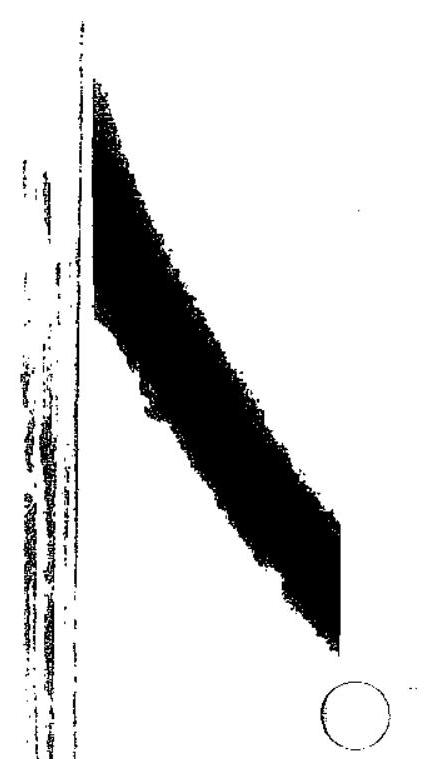
\includegraphics[max width=\textwidth]{2022_11_11_ca6a6c1a0324ee23e523g-38}\\
a. Methane\\
b. Carbon dioxide\\
c. Hydrogen sulfide\\
d. Manganese

\begin{enumerate}
  \setcounter{enumi}{3}
  \item Of the following types of extinguishers, which should be used on electrical fires?\\
a. Water\\
b. Soda-acid\\
c. Blanket\\
(d.) Carbon dioxide

  \item Wear safety goggles when\\
a. Handling acid\\
b. Doing paperwork\\
c. Driving trucks\\
d. Measuring turbidity

\end{enumerate}

\section{SAFETY AND EMERGENCY PREPAREDNESS}
\section{Sample Questions for Class 111 , answers on p. 94}
\begin{enumerate}
  \item The proper emergency repair kit for a ton chlorine cylinder is an\\
a. Emergency kit $A$\\
b. Emergency kit $\mathrm{B}$\\
c. Emergency kit C\\
d. Emergency kit T

  \item What is the only type of self-contained breathing apparatus that should be used at water plants?\\
a. Negative-pressure\\
b. Zero-pressure\\
c. Positive-pressure\\
d. Air-pressure

  \item The use of ammonia solution on a chlorine gas leak from the disinfection assembly may cause which of the following?\\
a. Explosion\\
b. Hydrochloric acid\\
c. Toxic gases\\
d. Dense white smoke

  \item Which of the following substances pose an immediate health threat whenever standards are exceeded?\\
a. Benzene and mercury\\
(b.) Coliform and nitrate\\
c. Mercury and coliform\\
d. Lead and nitrate

  \item Ozone contactors must have a system to collect ozone off-gas because ozone is\\
a. Toxic $10 \mathrm{ppb}$\\
b. Explosive\\
c. Mutagenic\\
d. Magnetic

\end{enumerate}

\section{SAFETY AND EMERGENCY PREPAREDNESS}
\section{Sample Questions for Class IV, answers on p. 95}
\begin{enumerate}
  \item What is the causative organism for cholera?\\
a. Vibrio\\
b. Shigella\\
c. Yersinia\\
d. Mycobacterium

  \item Which health effect category refers to an organic chemical that is a known carcinogen?\\
a. Category I\\
b. Category II\\
c. Category III\\
d. Category IV

\end{enumerate}


\includegraphics[max width=\textwidth]{2022_11_11_ca6a6c1a0324ee23e523g-40}

\begin{enumerate}
  \setcounter{enumi}{2}
  \item A room measures $12 \mathrm{ft}$ high, $30 \mathrm{ft}$ long, and $17 \mathrm{ft}$ wide. How many cubic feet per minute of air must a blower in an air exchange unit move to completely change the air every 10 minutes?\\
a. 102\\
b. 612\\
c. 1,020\\
d. 6,120

  \item One volume of liquid chlorine gas will expand, at room temperature and pressure, to occupy how many volumes of gas?\\
a. 16 volumes\\
b. 46 volumes\\
c. 460 volumes\\
d. 960 volumes

  \item What is the odor detection limit of chlorine gas?\\
a. $0.1 \mathrm{ppm}$\\
b. $0.3 \mathrm{ppm}$\\
c. $0.5 \mathrm{ppm}$\\
d. $1.0 \mathrm{ppm}$

\end{enumerate}

\section{PERFORM ADMINISTRATIVE DUTIES}
\section{Sample Questions for Class I, answers on p. 217}
\begin{enumerate}
  \item The SDWA defines a public water system that supplies piped water for human consumption as one that has\\
a. 10 service connection or serves 20 or more people for 60 or more days per year\\
b. 15 service connections or serves 20 or more people for 90 or more days per year\\
c. 10 service connections or serves 25 or more people for 30 or more days per year

  \item 15 service connections or serves 25 or more people for 60 or more days per year

  \item The most common water complaints are taste, odor, and\\
a. $\mathrm{pH}$ level\\
b. Faucet pressure\\
c. Colored water\\
d. Leaking pipes

  \item What US agency establishes drinking water standards?\\
a. AWWA\\
b. USEPA\\
c. NIOSH\\
d. NSF

  \item Why should the operator contact area companies with underground utilities before starting an underground repair job?\\
a. To determine if there have been recent excavations in that location\\
k. To ask the companies to locate and mark the location of their utilities in the area of the repair job\\
c. To determine if they also have excavating to do in the area\\
d. To ask if they will help route traffic while you are doing the repair job\\

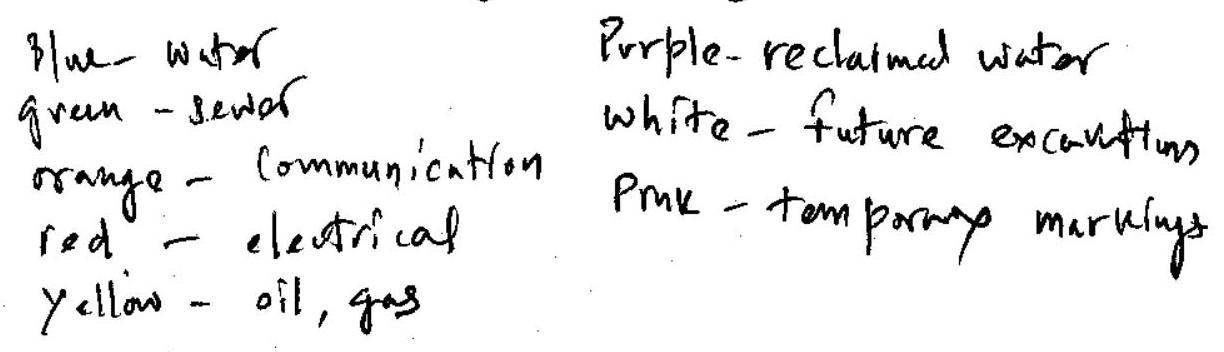
\includegraphics[max width=\textwidth]{2022_11_11_ca6a6c1a0324ee23e523g-41}

\end{enumerate}

\section{MCAMON STUDY CUIDE}
\begin{enumerate}
  \setcounter{enumi}{4}
  \item According to the USEPA regulations, the owner or operator of a public water system that fails to comply with applicable monitoring requirements must give notice to the public within\\
a. 1 week of the violation in a letter hand-delivered to customers
\end{enumerate}

b. 45 days of the violation by posting a notice at the town hall

(c.) 3 months of the violation in a daily newspaper in the area\\
served by the system

a. I year of the yiolation by inclinling a letter writh the water bill

\section{PERFORM ADMINISTRATIVE DUIIES}
Sample Questions for Class II, answers on p. 218

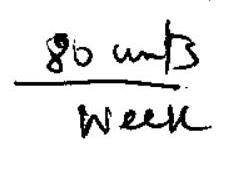
\includegraphics[max width=\textwidth]{2022_11_11_ca6a6c1a0324ee23e523g-43}\\
lowech rostre $+4$ wevesto abtan wewsiftlo $14 \times 80$

\begin{enumerate}
  \item Your departmont uses 80 units of an item per week. You are required to maintain a 10 week roserve of this.item at all times and it requires 4 weeks to obtain a new supply. What is the minimum reorder point?\\
a. 320 units\\
b. 800 units\\
c. 1,120 irnits\\
d. 2,240 units
\end{enumerate}

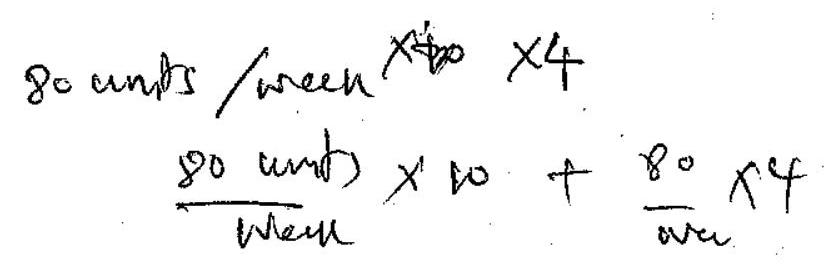
\includegraphics[max width=\textwidth]{2022_11_11_ca6a6c1a0324ee23e523g-43(1)}

\begin{enumerate}
  \setcounter{enumi}{1}
  \item What is the maximum contaminant level gnal for chloride?\\
a. $2.5 \mathrm{mg} / \mathrm{l}$,\\
b. $25 \mathrm{mg} / \mathrm{L}$\\
c. $250 \mathrm{mg} / \mathrm{L}$\\
d. $2,500 \mathrm{mg} / \mathrm{L}$
\end{enumerate}

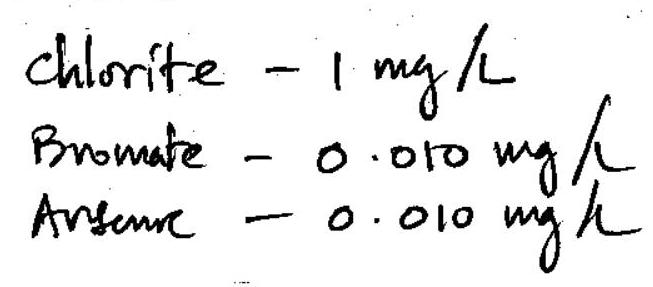
\includegraphics[max width=\textwidth]{2022_11_11_ca6a6c1a0324ee23e523g-43(2)}

\begin{enumerate}
  \setcounter{enumi}{2}
  \item What is the median value of the following data: $100,300,580,250,275$, 335,580\\
a. 250\\
(b.) 300
\end{enumerate}

$100200,275,300,3.35,580,580$

\begin{enumerate}
  \setcounter{enumi}{3}
  \item The National Primary Drinking Water Regulations apply to drinking water contaminants that may have adverse effects on\\
a. Water color\\
b. Water taste\\
c. Water odor\\
d. Human health
\end{enumerate}

-5. Which of the following is considered an acute risk to bealth?\\
a. Two Tier 2 violations\\
b. One Tier 2 violation\\
c. Two Tier 1 violations\\
d. One Tier 1 violation

\section{ERFORM ADMINISTRATIVE DUTIES}
\section{Sample Questions for Class Ill, answers on p. 219}
\begin{enumerate}
  \item Records on turbidity analyses should be kept for a minimum of\\
(a.) 5 years\\
c. 10 years\\
i. 25 years

  \item What is the difference between a primary standard and a secondary standard?

\end{enumerate}

a. Primary standards refer to substances that are carcinogenic, secondary standards do not

b. Primary standards refer to substances that are thought to

\begin{itemize}
  \item pose a threat to human health, secondary standards do not
\end{itemize}

c. Primary standards refer to substances that, if not put in check, will eventually kill humans, secondary standards do not

d. Secondary qualities are aesthetic qualities and will only make some people sick, while primary standards refer to substances that will make everyone sick and may possibly cause death

\begin{enumerate}
  \setcounter{enumi}{2}
  \item An employee receives an hourly wage of $\$ 13.25$ plus overtime pay of $1.5$ times the hourly wage. Overtime pay is given for each hour worked over 40 hours per week. If an employee works 48 hours during a week, what is the compensation before taxes?\\
a.) $\$ 159.00$\\
b. $\$ 530.00$\\
530\\
c. $\$ 689.00$\\
d. $\$ 848.00$

  \item What type of computer software is recommended for maintaining records such as turbidity levels?\\
a. Word processor\\
b. E-mail\\
c. Graphics\\
d. Database 5. How should a supervisor handle a recurring problem with an operator?\\
a. Document the problem in writing and talk to the operator\\
b. Promote the operator so he develops a better work ethic\\
c. Ask a co-worker to discuss the problem with the operator\\
d. Ignore the situation; problems tend to work themselves ont

\end{enumerate}

\section{ERFORM ADMIIISTRATIVE DUTIES}
\section{Sample Questions for Class IV, answers on p. 220}
\begin{enumerate}
  \item Records on bacteriological analyses should be kept for a minimum of\\
a. 5 years\\
b. 7 years\\
c. 10 years\\
d. 25 years

  \item What should a supervisor do if an employee is performing work in an unsafe manner?\\
a. Discuss the incident with the employee during the iaxi performance appraisal\\
b. Stop the work immediately and train the employee to perform the work safely\\
c. Call OSHA immediately to investigate the incident\\
d. Give the employee a written warning that the work was performed unsafely

  \item Your plant's current annual budget for salaries is $\$ 450,000$. A. $3 \%$ raise will be given to all employees next year. Calculate the salary budget for next year.\\
a. $\$ 463,500$\\
$\overrightarrow{\text { b. }} \$ 470,000$\\
c. $\$ 483,500$.\\
d. $\$ 490,000$

  \item What is the action level for lead?\\
a. $0.01 \mathrm{mg} / \mathrm{L}$\\
(b) $0.015 \mathrm{mg} / \mathrm{L}$\\
c. $0.1 \mathrm{mg} / \mathrm{L}$\\
d. $0.5 \mathrm{mg} / \mathrm{L}$

  \item How must water systems serving a population over 10,000 distribute the consumer confidence report to customers?\\
a. Television announcement\\
b. Radio announcement\\
c. Public meeting\\
(d.) Mail

\end{enumerate}

\section{TTOR WATER QUALTTY}
\section{Sample Questions for Class Il, answers on p. 202}
\begin{enumerate}
  \item What is the recommended minimum contact time when disinfecting water mains with the chlorine slug method?\\
a. 3 hours\\
b. 6 hours\\
c. 10 hours\\
d. 12 hours

  \item Which of the following best defines the term static water level?\\
a. Water level in a well after a pump has operated for a period of time\\
b. Water level in a well when the well is not in operation\\
c. Water level in a well measured from the ground surface to the drawdown water level\\
d. Waterelevel in a well measured from the natural water level to the drawdown water level

  \item Where are chlorine samples typically collected from in the distribution system?\\
a. At points representative of conditions within the system\\
b. Uniformly distributed throughout the system as much as possible\\
c. At the extreme locations of the system\\
d. At representative points throughout the system based on elevation

  \item Which of the following best defines the cone of depression?\\
a. Change in water elevation from the normal level to the pumping level\\
b. Depression around the well of the water surface caused by pumping water from the well\\
c. Water level in a well after a pump has operated over a period of time\\
d. Measured distance from the ground to the pumping level

  \item Turbidity is caused by\\
a. Dissolved solids\\
b. Suspended particles\\
c. Dissolved gases\\
d. Dissolved colored solids

\end{enumerate}

\section{MONITOR WATER QUALITY}
\section{Sample Questions for Class I, answers on p. 201}
\begin{enumerate}
  \item As the temperature of the water increases, the disinfecting action of chlorine is\\
a. More effective\\
b. Not affected\\
c. Less effective\\
d. Likely to increase DO

  \item Large fill stingage tanks aro typienlly disinfoctod with a chlorine? residual of\\
a. $3 \mathrm{mg} / \mathrm{L}$\\
b. $\quad 10 \mathrm{mg} / \mathrm{L}$\\
c. $25 \mathrm{mg} / \mathrm{L}$\\
d. $50 \mathrm{mg} / \mathrm{L}$

  \item Why is a well acidified?\\
a. Take out soluble iron or manganese\\
b. Increase the well's productivity\\
c. Remove objectionable gases\\
d. Rsmova turbidity

  \item What is the primary source of coliforms in a water supply?\\
a. Insects that live or die in the water source\\
b. Protozoans and other microorganisma\\
c. Fertilizers\\
d. Fecal material from warm-blooded animals

\end{enumerate}

B. $\mathrm{DH}$ in measure of\\
a. Conductivity\\
b. Water ability to neutralize acid\\
c. Hydrogen ions\\
d. Dissolvad solds

\section{MONITOR WATER QUALIIY}
Sample Class Ill Ounestions, answers on p., 203

\begin{enumerate}
  \item What is the term for water samples collected at regular intervals
\end{enumerate}

a. Time grab samples

b. Time flow samples

c. Time composite samples

d. Proportional time composite samples

\begin{enumerate}
  \setcounter{enumi}{1}
  \item What chemical is present in a bacteria sample bottle for the purpose of neutralizing chlerine?\\
a. Sodium benzato\\
b. Sodium thiosulfate\\
c. Sodium phenoxide\\
d. Sodium salicylate

  \item 
  \begin{itemize}
    \item Chlorine neutralization is necessary when a treated water sample is to be analyzed for\\
a. Iron\\
b. Bacteria\\
c. Manganese\\
d. Nitrater
  \end{itemize}
  \item The residual drawdown of a well is defined as

\end{enumerate}

a. Water level in a well after a pump has operated over a perind

b. Measured

c. Water level below the normal level that persists after a

c. Water level below the normal level that persists after a\\
well pump has been off for a period of time\\
d. Measured distance between the water level and the top of the\\
screen

.5. What is the basis for the number of samples that must be collected for utilities monitoring for lead and copper that are in compliance or have installed corrosion control?\\
a. Size of distribution system\\
b. Population\\
c. Amount of water produced\\
d. Number of raw water sources

\section{R WATER QUALITY}
\section{Sample Class IV Questions, answers on p. 204}
\begin{enumerate}
  \item Where should bacteriological samples be collected in the distribution system?
\end{enumerate}

a. Uniformly distributed throughout the system based on area

b. At locations that are representative of conditions within the system

c. Almost always from extreme locations in the system but occasionally at other locations

d. Uniformly throughout the system based on population density

\begin{enumerate}
  \setcounter{enumi}{1}
  \item The quantity of oxygen that can remain dissolved in water is related to\\
a. Temperature\\
b. $\mathbf{p H}$\\
c. Turbidity\\
d. Alkalinity.

  \item In coliform analyses using the presence-absence test, a sample should be incubated for\\
a. 24 hours at $25^{\circ} \mathrm{C}$\\
b. 36 hours at $35^{\circ} \mathrm{C}$\\
c. 24 and 36 hours at $25^{\circ} \mathrm{C}$\\
d. 24 and 48 hours at $35^{\circ} \mathrm{C}$

  \item What is the potential cross-connection hazard from sprinkler systems?\\
a. Low\\
b. Low to moderate\\
c. Moderate\\
d. High

  \item A well produces $365 \mathrm{gpm}$ with a drawdown of $22.5 \mathrm{ft}$. What is the specific yield in gallons per minute per foot?

  \item $16.2$\\
b. $22.5$\\
c. $32.4$\\
d. $36.5$

\end{enumerate}

\section{IDDITIONAL SAMPLE QUESTIONS, answers on p. 100}
\begin{enumerate}
  \item What is the ratio of lime to copper sulfate for controlling algae growth on basin walls?\\
(a.) 1 part lime to 1 part copper sulfate\\
b. 1 part lime to 2 parts copper sulfate\\
c. 1 part lime to 3 parts copper sulfate\\
d. 2 parts lime to 3 parts copper sulfate

  \item Copper sulfate is used in surface water reservoirs to control\\
a. Emergent weeds\\
b. Algae\\
c. Mosquito larvae\\
d. Snails

  \item Which is the correct order (on the average) from smallest to largest for the microorganisms below?\\
a. Giardia cysts, bacteria, viruses\\
(b.) Viruses, bacteria, Giardia cysts\\
c. Bacteria, Giardia cysts, viruses\\
d. Giardia cysts, viruses, bacteria hrghor the log remoral smaller the \$ize of the mrroorgarsm

\end{enumerate}

$$
\begin{array}{ll}
\text { virul-4 log } & 99.99 \\
\text { grantion }-2.5-3 \text { log } & 9.9-9
\end{array}
$$

\begin{enumerate}
  \setcounter{enumi}{3}
  \item What is the usual strength of sodium hypochlorite, i.e., available chlorine?\\
a. 5 to $15 \%$\\
b. 45 to $50 \%$\\
c. 65 to $70 \%$\\
d. 80 to $85 \%$
\end{enumerate}

$$
\begin{aligned}
&\mathrm{NaOCl}-12.5 \% \\
&\mathrm{Ca}(\mathrm{OCl})_{2}-65 \mathrm{Y}
\end{aligned}
$$

\begin{enumerate}
  \setcounter{enumi}{4}
  \item Calcium hypochlorite (71.5 percent available chlorine) is used to treat $5.8$ $\mathrm{mgd}$. If $237 \mathrm{lb} /$ day of calcium hypochlorite is used, what is the chlorine dosage in milligrams per liter?\\
a. $1.7 \mathrm{mg} / \mathrm{L}$\\
b. $3.5 \mathrm{mg} / \mathrm{L}$ $237 \times 0.715$\\
c. $5.8 \mathrm{mg} / \mathrm{L}$\\
d. $16.9 \mathrm{mg} / \mathrm{L}$
\end{enumerate}


\includegraphics[max width=\textwidth]{2022_11_11_ca6a6c1a0324ee23e523g-52}

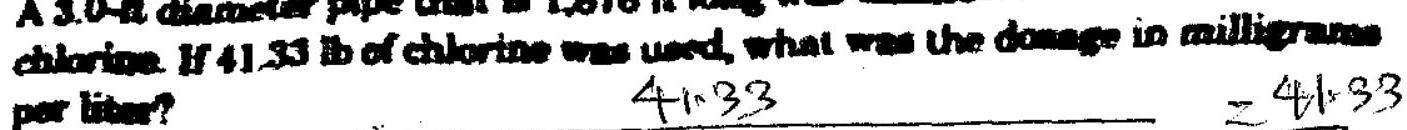
\includegraphics[max width=\textwidth]{2022_11_11_ca6a6c1a0324ee23e523g-52(1)}

a. $18 m \sin ^{2}$

b. 412

$\therefore c 0 \mathrm{ma}$

d. 99

$49.97$

\begin{enumerate}
  \setcounter{enumi}{6}
  \item Tritahmothanes are usualy anseciated with
\end{enumerate}

a High levels of atae in a surfice water soure

b. Surfor water high to or andus

$\dot{x}_{2}$ Watler with angunt that han


\includegraphics[max width=\textwidth]{2022_11_11_ca6a6c1a0324ee23e523g-52(2)}


\includegraphics[max width=\textwidth]{2022_11_11_ca6a6c1a0324ee23e523g-52(3)}

\begin{itemize}
  \item Onime
\end{itemize}

b. Untavialat 1 int

\begin{itemize}
  \item Charito elutio
\end{itemize}

d. Sollion charible


\includegraphics[max width=\textwidth]{2022_11_11_ca6a6c1a0324ee23e523g-52(4)}\\
chtains diristretem?

2 Tarsiut

b. Color

c. Radon

a. Carboa diaride

\begin{enumerate}
  \setcounter{enumi}{9}
  \item Which of the fallowing forme of chlorine has no divinfecting capacity?
\end{enumerate}

a Fypochlorous acid

b. Hydrochloric acid

c. Hypochlorite ion

d. Dichloramize

\begin{enumerate}
  \setcounter{enumi}{10}
  \item Find the detention time in minutes for a clarifier that has a diameter of $152 \mathrm{ft}$ and a water depth of $8.22 \mathrm{ft}$, if the flow rate is $6.8 \mathrm{mgd}$.\\
a. 32 minutes\\
b. 236 minutes\\
c. 775 minutes\\
d. 5,604 minutes
\end{enumerate}

$$
\begin{aligned}
\frac{1.115 M G}{\frac{6.8 M G}{D *}} &=0.16 \text { Doys } \\
&=236 \mathrm{~m} n
\end{aligned}
$$

\begin{enumerate}
  \setcounter{enumi}{11}
  \item A plant is treating water at $21.3 \mathrm{mgd}$. If lime is being added at a rate of
\end{enumerate}

$$
\begin{array}{lll}
\text { WATER TREATMENT } & 41 & 21.3 \mathrm{MGT} \\
& 0.6
\end{array}
$$

$417.16 \mathrm{~g} / \mathrm{min}$, what is the lime dosage in milligrams per liter?\\
(a.) $7.43 \mathrm{mg} / \mathrm{L}$\\
b. $8.34 \mathrm{mg} / \mathrm{L}$\\
c. $19.6 \mathrm{mg} / \mathrm{L}$\\
d. $21.3 \mathrm{mg} / \mathrm{L}$


\includegraphics[max width=\textwidth]{2022_11_11_ca6a6c1a0324ee23e523g-53}

$M G D=21.3 M G D$ $12.78$

\begin{enumerate}
  \setcounter{enumi}{17}
  \item A raw water flow of $17 \mathrm{cfs}$ is prechlorinated with $285 \mathrm{lb}$ of chlorine gas. If the flow is changed to $28 \mathrm{cfs}$, what should the adjustment be to the chlorinator?\\
a. $17 \mathrm{lb}$ of $\mathrm{Cl}_{2} 28$\\
b. $\quad 28 \mathrm{lb}$ of $\mathrm{Cl}_{2}$\\
c. $285 \mathrm{lb}$ of $\mathrm{Cl}_{2}$\\
d. $470 \mathrm{lb}$ of $\mathrm{Cl}_{2}$
\end{enumerate}

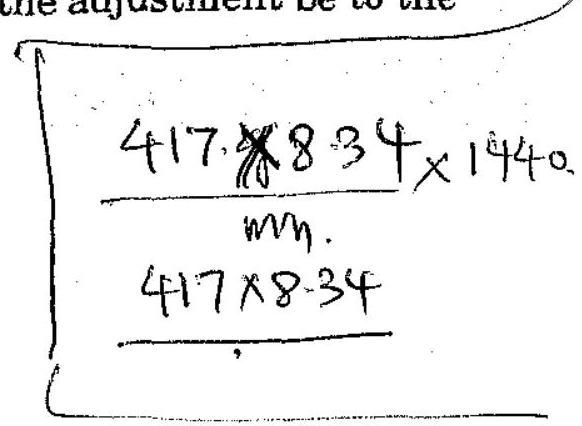
\includegraphics[max width=\textwidth]{2022_11_11_ca6a6c1a0324ee23e523g-53(1)}

\begin{enumerate}
  \setcounter{enumi}{13}
  \item An operator mixes $40 \mathrm{lb}$ of lime in a 100 -gal tank that contains 80 gal of water. What is the percent of lime in the slurry?\\
a. $3 \%$\\
b. $6 \%$\\
c. $9 \%$\\
d. $12 \%$
\end{enumerate}

$$
\frac{40}{667+40}=\frac{40}{874}
$$

1321 $\frac{417 \mathrm{~g}}{8.34}$


\includegraphics[max width=\textwidth]{2022_11_11_ca6a6c1a0324ee23e523g-53(2)}

\begin{enumerate}
  \setcounter{enumi}{14}
  \item Red water may be caused by iron concentrations above\\
a. $0.01 \mathrm{mg} / \mathrm{L}$\\
b. $\quad 0.03 \mathrm{mg} / \mathrm{L}$\\
c. $0.1 \mathrm{mg} / \mathrm{L}$\\
d. $0.3 \mathrm{mg} / \mathrm{L}$
\end{enumerate}

Black water $=0.05$ Manganuse Absorbtion

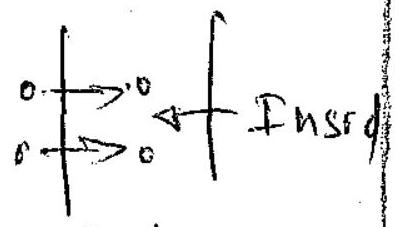
\includegraphics[max width=\textwidth]{2022_11_11_ca6a6c1a0324ee23e523g-53(3)}

\begin{enumerate}
  \setcounter{enumi}{15}
  \item Which of the following best defines adsorption?
\end{enumerate}

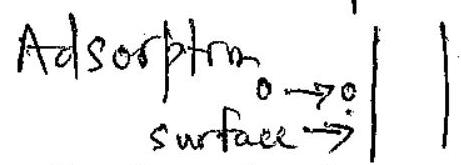
\includegraphics[max width=\textwidth]{2022_11_11_ca6a6c1a0324ee23e523g-53(4)}

a. Assimilation of one substance into the body of another by molecular or chemical action

b. Adhesion of a gas, liquid, or dissolved substance onto the surface or interface zone of another substance

c. Converting small particles of suspended solids into larger particles by the use of chemicals

d. Chemical complexing of metallic cations with certain inorganic compounds 17. Hard water scale is usually caused by\\
a. Calcium bicarbonate\\
b. Calcium carbonate\\
c. Magnesium bicarbonate\\
d. Magnesium carbonate

\begin{enumerate}
  \setcounter{enumi}{17}
  \item About how much alkalinity is required for each milligram per liter of alum added to raw water?\\
(a.) $0.5 \mathrm{mg} / \mathrm{L}$\\
b. $1.0 \mathrm{mg} / \mathrm{L}$\\
c. $1.5 \mathrm{mg} / \mathrm{L}$\\
d. $2.0 \mathrm{mg} / \mathrm{L}$

  \item A water treatment plant's flocculation-coagulation and sedimentation processes should be checked if which of the following changes?\\
a. Turbidity\\
b. Chlorine feed rate\\
c. Fluoride feed rate\\
d. Total trihalomethanes

  \item Which of the following is an example of a weighting agent?\\
a. Polyelectrolytes\\
b. Bentonite clay\\
c. Calcium carbonate\\
d. Sodium bicarbonate

  \item Algae can shorten filter runs by\\
a. Clogging the filters\\
b. Increasing chlorine demand\\
c. Lowering the $\mathrm{pH}$\\
d. Increasing turbidity

  \item Coagulation is a chemical and physical reaction that converts\\
a. Settleable solids into nonsettleable solids\\
b. Nonsettleable solids into settleable solids\\
c. Dissolved solids into settleable solids\\
d. Dissolved solids into a precipitate 28. Water corroston in metal piping will increase if\\
a. The pH is above 7,0 and has low dissolved oxygen levels\\
b. The slkalinity is high and water temperature is low\\
c. Total dissolved solids are high and the $\mathrm{pH}$ is below $7.0$\\
d. The $\mathrm{pH}$ and alkalinity increase

  \item What is schmutzdecke?

\end{enumerate}

a. Settled floc material in a sedimentation basin

(b.) Fine sand and a sticky mat of suspended matter that forms on the surface of a sand filter

c. Adsorption of divalent metal ions onto the surfaces of resins used in ion exchange

d. Thin layer of protection formed on the inside of metal pipes by the reaction between the alkalinity in the water and zinc orthophosphate

\begin{enumerate}
  \setcounter{enumi}{24}
  \item What is the cathode? Cattode - Negatrix Avocle - positrive
\end{enumerate}

a. Negative pole of an electrolytic cell or system

b. Positive pale of an electrolytic cell or system

c. Negative pole of a polyelectrolyte

Anrme - Negative Catione - Posritine.

d. Positive pole of a polyelectrolyte

\begin{enumerate}
  \setcounter{enumi}{25}
  \item What metals are moet likely to leach from household plumbing and cause a health haxard?\\
a. Iron and sine\\
b. Iron and copper\\
c Irex and lend\\
d. Copper and basd
\end{enumerate}

\section{The for rate over conventional sedimentation besins in commonly deninudi not to enced}
. 12003 ha

\begin{enumerate}
  \item $20,00020 \pi a x$
\end{enumerate}

\begin{itemize}
  \item 101,038
\end{itemize}

\begin{enumerate}
  \setcounter{enumi}{3}
  \item 260,090 ginta 28. If poorly formed floc is leaving the settling basin, which of the following should be done?\\
a. Stop the mixer\\
b. Increase the coagulant or add a coagulant aid\\
c. Increase filter run time\\
d. Decrease the chlorination rate

  \item Slow sand filters are cleaned by\\
a. Air and water backwash\\
b. Water backwash alone\\
c. Scraping about 1 in. of sand off the top\\
d. Surface wash

  \item What is the most common filtration rate for slow sand filters?\\
a. $0.02 \mathrm{gpm} / \mathrm{sq} \mathrm{ft}$\\
(b.) $0.05 \mathrm{gpm} / \mathrm{sq} \mathrm{ft}$\\
c. $\quad 0.1 \mathrm{gpm} / \mathrm{sq} \mathrm{ft}$\\
d. $\quad 0.5 \mathrm{gpm} / \mathrm{sq} \mathrm{ft}$

  \item Which of the following do long filter runs tend to cause?\\
a. Air binding\\
(b.) Slime growths\\
c. Mud balls.\\
d. Media loss

\end{enumerate}

Surface boding $=$

$$
\begin{aligned}
&\text { Plow rate (gpw) } \\
&\text { Area }(s q p)
\end{aligned}
$$

\begin{enumerate}
  \setcounter{enumi}{31}
  \item A water treatment plant has six filters with an average flow rate of $6.1 \mathrm{gpm} / \mathrm{sq} \mathrm{ft}$. If the plant flow is $70 \mathrm{cfs}$, what is the filtration area of each filter?\\
a. 686 sq ft\\
(b.) $861 \mathrm{sq} \mathrm{ft}$\\
c. $2,060 \mathrm{sq} \mathrm{ft}$\\
d. $5,553 \mathrm{sq} \mathrm{ft}$\\

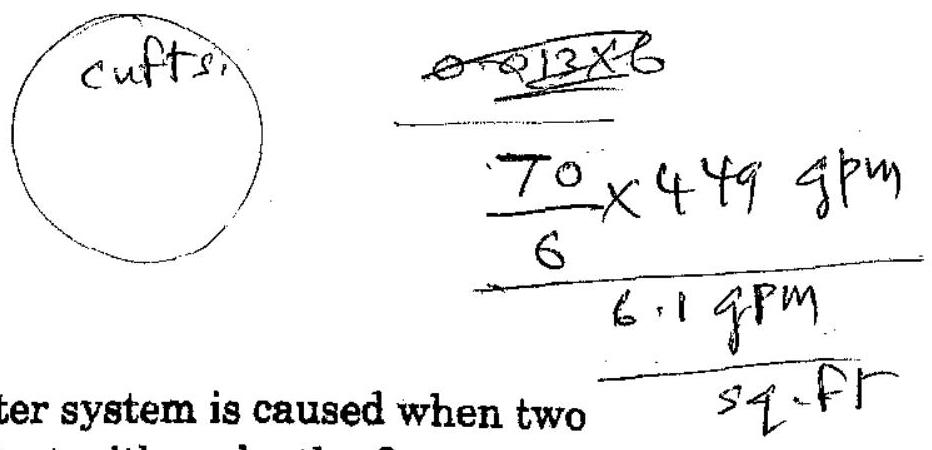
\includegraphics[max width=\textwidth]{2022_11_11_ca6a6c1a0324ee23e523g-56}\\
different metals come into contact with each other?\\
a. Concentration cell corrosion\\
b. Uniform corrosion\\
c. Galvanic corrosion\\
d. Stray current corrosion 34. When should ammonia be added to the water when making disinfectant chloramines to improve disinfection?\\
a. Before the chlorine is added\\
b. After the chlorine is added\\
c. During filtration\\
d. Before filtration

  \item Alum and ferric sulfate may have poor coagulation due to\\
a. High turbidity in the water\\
b. Low color in the water\\
c. High color in the water\\
d. Low alkalinity in the water

  \item The process of cathodic protection can be used to reduce or prevent corrosion by protecting metal parts exposed to\\
a. Soil\\
b. Chloramine\\
c. Permafrost\\
d. Excessive turbidity

  \item Which of the following disinfectants is usually generated on-site?\\
a. Chlorine gas\\
b. Potassium permanganate\\
c. Chlorine dioxide\\
d. Sodium hypochlorite

  \item If too much potassium permanganate is used to treat water\\
a. The sodium level will increase\\
b. Disinfection will not be necessary\\
c. All contaminants are removed\\
Sulfate: $\mathrm{SO}_{4}{ }^{2-}{ }^{2-}$.\\
d. The water turns pink

  \item Which of the following chemicals can be activated for use as a coagulant aid with alum?

\end{enumerate}

$$
\mathrm{Na}_{2} \mathrm{~S}_{2} \mathrm{O}_{3} \text { - Sod rump frosuffate. }
$$

a. Calcium silicate Cas S4 Oq\\
b. Sodium silicate $=\mathrm{Na}_{2} \mathrm{~S}_{4} \mathrm{O}$\\
c. Sodium hypochlorite

\begin{itemize}
  \item Maocl\\
d. Calcium hypochlorite\\
$(a \operatorname{loc})_{2}$ 4U. In conventional coagulation, the average time to develop heavy floc particles is?\\
a. 1 minute\\
b. 10 minutes\\
c. 30 minutes\\
d. 60 minutes
\end{itemize}

\begin{enumerate}
  \setcounter{enumi}{40}
  \item Which of the following is a difference between conventional filters and greensand filters?\\
a. Greensand grains are larger than conventional silica grains\\
b. Greensand filters remove iron and manganese by adsorption and oxidation\\
c. Conventional filters remove iron and manganese by adsorption and oxidation\\
d. Conventional beds must be regenerated during backwash

  \item Under heavy loading, head loss on a manganese greensand filter quickly becomes excessive because\\
a. Greensand grains are smaller than silica sand\\
b. Greensand filters are smaller than conventional filters\\
c. Greensand filters are not backwashed\\
d. Greensand filter runs are longer than conventional filter runs

  \item The filter medium in DE filters is\\
a. Dielectric earth\\
b. Diatomaceous earth\\
c. Deionized earth\\
d. Disinfected earth

  \item Which of the following is a required treatment technique for the control of lead?\\
a. Ion exchange\\
b. Corrosion control\\
c. Lime softening\\
d. Activated carbon 45. Bar screens are used to\\
a. Remove turbidity\\
b. Remove debris\\
c. Cover pipes\\
d. Size sand

  \item Which of the following factors affects the settling rate of particles?\\
a. Particle size\\
b. Clarifier circumference\\
c. Filter surface loading rate\\
d. Method of prechlorination

  \item Coagulation processes rely on\\
a. High-quality water\\
b. Higher velocities\\
c. Filter valves\\
d. The formation of large settleable particles

  \item Which of the following substances is the most effective disinfection residual?\\
a. Trichloramine\\
b. Hypochlorous acid\\
c. Chloramine\\
d. Hypochlorite ion\\

\includegraphics[max width=\textwidth]{2022_11_11_ca6a6c1a0324ee23e523g-59}

  \item Water is flowing at a velocity of $1.70 \mathrm{fps}$ in a 10 -in. diameter pipe. $) 1.7 \times \frac{10}{12} \times 10 \times 0.7872$\\
If the pipe changes from the 10 -in. to a 6-in. pipe, what will the velocity be in the 6-in. pipe?\\
a. $2.8 \mathrm{fps}$\\
b. $4.6 \mathrm{fps}$\\
c. $10.2 \mathrm{fps}$\\
d. $35.3 \mathrm{fps}$

\end{enumerate}

$$
1.7 \times \frac{10}{12} \times 10 \times 0.785=0.4267
$$

\includegraphics[max width=\textwidth]{2022_11_11_ca6a6c1a0324ee23e523g-59(1)}

\begin{enumerate}
  \setcounter{enumi}{49}
  \item Which type of solution contains 1 gram equivalent weight of a reactant compound per liter of solution?\\
a. Molar solution\\
b. Molal solution\\
c. Normal solution\\
d. Percentage strength solution
\end{enumerate}

$$
\begin{aligned}
&\text { Normal solutim - } 1 \text { grm /litar } \\
&\text { Porcentge " }-2 \text { grm/1ttf } \\
&\text { Molor " - Molor wruaht solut }
\end{aligned}
$$

\begin{enumerate}
  \setcounter{enumi}{50}
  \item What term describes a measure of the capacity of water to neutralize strong acids?\\
a. Acidity\\
b. Alkalinity\\
c. Hardness\\
d. $\mathrm{pH}$

  \item What piece of laboratory glassware is primarily used to mix chemicals and measure approximate volumes?\\
(a.) Beaker - approximate volume\\
b. Pipet - trandort a measued of bqual.\\
c. Buret = drtution\\
d. Graduated cylinder - preeighy mentme volumetrr Flakk - Most preerse

  \item What laboratory device sterilizes laboratory apparatus and microbial media by using pressurized steam?\\
a. Muffle furnace\\
b. Aspirator\\
c. Autoclave\\
d. Membrane filter

  \item Which of the following chemicals cause alkalinity in water?\\
a. Calcium carbonate and calcium oxide\\
b. Calcium sulfate and sodium sulfate\\
c. Magnesium chloride and iron chloride\\
d. Sodium chloride and calcium chloride

  \item What should the sample volume be when testing for total coliform bacteria?\\
a. $100 \mathrm{~mL}$\\
b. $250 \mathrm{~mL}$\\
c. $500 \mathrm{~mL}$\\
d. $1,000 \mathrm{~mL}$ s6. Primary drinking water standarda require Giardia removal at\\
a. Two log (99. ()\% $\%$\\
b. Throe $\log (99.9 \%)$\\
c. Four $\log (90.99 \%)$\\
d. Five log $(99.999(\%)$

\end{enumerate}

\includegraphics[max width=\textwidth]{2022_11_11_ca6a6c1a0324ee23e523g-61}

B7. Recarbonation basins are used to stabilize water after\\
a. ITiliration\\
b. Disinfection\\
c. Softening\\
d. Oodiuladion

addrm $\mathrm{Co}_{2}$ to taner bh. Since softing incrase ph by $\operatorname{lime}[\operatorname{col}(\mathrm{ct}) 2]$

\begin{enumerate}
  \setcounter{enumi}{67}
  \item The least reactive metals are called\\
a. Anodic metals\\
b. Cathodic metals\\
c. Galvanic metals\\
d. Tempered metals

  \item What precipitate is formed in alum coagulation?\\
"a. Aluminum hydroxide

\end{enumerate}

\begin{itemize}
  \item Floc\\
b. Complex organo-aluminum compounds\\
c. Complex sulfate compounds and aluminum salts\\
d. Aluminum salts and organo-sulfate compounds
\end{itemize}

\begin{enumerate}
  \setcounter{enumi}{59}
  \item Autoclaving will sterilize\\
a. At high temperatures near $600^{\circ} \mathrm{C}$\\
b. With ultraviolet light\\
c. With steam at $121^{\circ} \mathrm{C}$ and 15 psi\\
d. With chlorine gas

  \item What is the most common method used to determine if water is close to the equilibrium point?\\
a. Marble test\\
b. Langelier index\\
c. Temperature\\
d. Dissolved oxygen 62. Which of the following is used to determine compliance for total coliforms?\\
(a.) Most probable number procedure\\
b. Coliforms per $100 \mathrm{~mL}$\\
c. Presence-absence method\\
d. Heterotrophic plate count

  \item What is the percent potassium $(K)$ by weight in potassium permanganate $\left(\mathrm{KMnO}_{4}\right)$ ?\\
a. $24.742 \%$\\
b. $39.102 \%$\\
c. $54.938 \%$\\
d. $63.998 \%$

  \item Small and medium-size utilities are considered to have optimal corrosion control if they meet the lead and copper action levels for\\
a. One sampling period\\
b. Two consecutive sampling periods\\
c. Three consecutive sampling periods\\
d. Four consecutive sampling periods

  \item What is pressure head caused by?\\
a. Water flow\\
b. Water pressure\\
c. Water elevation\\
d. Gauge pressure

\end{enumerate}

Motor Horse Power $\times$ Mator $\% \times$ punp $\%$

\includegraphics[max width=\textwidth]{2022_11_11_ca6a6c1a0324ee23e523g-62}

\begin{enumerate}
  \setcounter{enumi}{65}
  \item What is the motor horsepower ( $\mathrm{mhp}$ ) required if $200 \mathrm{hp}$ is required to move water with a pump with a motor efficiency of $88 \%$ and a pump efficiency of $81 \%$ ? NOTE: The $200 \mathrm{hp}$ in this problem is called the water horsepower (whp). The water horsepower is the actual energy (horsepower) available to pump water.\\
a. $166 \mathrm{mhp}$\\
b. $200 \mathrm{mhp}$\\
c.) $281 \mathrm{mhp}$\\
d. $355 \mathrm{mhp}$
\end{enumerate}

\includegraphics[max width=\textwidth]{2022_11_11_ca6a6c1a0324ee23e523g-62(1)}

2

\includegraphics[max width=\textwidth]{2022_11_11_ca6a6c1a0324ee23e523g-62(2)}

\begin{enumerate}
  \setcounter{enumi}{66}
  \item The flow of electrical current is measured in\\
a. Amperes\\
b. Ohms\\
c. Volts\\
d. Watts

  \item Unless water cooled, the operating temperature of a mechanical seal in a pump should never exceed\\
a. $95^{\circ} \mathrm{F}\left(35^{\circ} \mathrm{C}\right)$\\
b. $120^{\circ} \mathrm{F}\left(49^{\circ} \mathrm{C}\right)$\\
c. $140^{\circ} \mathrm{F}\left(60^{\circ} \mathrm{C}\right)$\\
d. $160^{\circ} \mathrm{F}\left(71^{\circ} \mathrm{C}\right)$

\end{enumerate}

\includegraphics[max width=\textwidth]{2022_11_11_ca6a6c1a0324ee23e523g-63}

\begin{enumerate}
  \setcounter{enumi}{68}
  \item The level in a storage tank (clear well) rises $3.1 \mathrm{ft}$ in $4.5$ hours. If the tank has a diameter of $225 \mathrm{ft}$ and the plant is producing $32.4 \mathrm{mgd}$, what is the average discharge rate of the treated water discharge pumps in gallons per minute?
\end{enumerate}

\includegraphics[max width=\textwidth]{2022_11_11_ca6a6c1a0324ee23e523g-63(1)}

\begin{enumerate}
  \setcounter{enumi}{69}
  \item What term describes the condition that exists when the source of the water supply is below the centerline of the pump?\\
a. Pressure head\\
b. Velocity head\\
c. Suction lift\\
d. Total discharge head
\end{enumerate}

$6,075,000$

\begin{enumerate}
  \setcounter{enumi}{70}
  \item One horsepower is equal to how many foot-pounds per minute?\\
a. 746\\
b. 3,300\\
c. 7,460\\
d. 33,000 72. What is the pressure reading at the discharge side of a pump that is pumping against a total head of $100 \mathrm{ft}$ ?\\
a. $2.3 \mathrm{psi}$\\
b. $4.3 \mathrm{psi}$\\
c. $23.1 \mathrm{psi}$\\
d. $\quad 43.3 \mathrm{psi}$

  \item What is the most common use today for a positive-displacement pump?\\
a. Raw water intake pump\\
b. System booster pump\\
c. Chemical feed pump\\
d. Filter feed pump

  \item What is the purpose of a bypass valve on a larger size gate valve?\\
a. Connect a new main to an existing main\\
b. Reduce pressure across both sides to ease opening and closing\\
c. Increase flow through the main line\\
d. Allow easy location of the main valve

  \item A corrosion-resistant pipe is used to carry the chlorine gas solution from the chlorine injector to the point of application because the $\mathrm{pH}$ range of the solution is\\
a. 0-1 standard units\\
b. 2-4 standard units\\
c. 6-8 standard units\\
d. 9-11 standard units

  \item Calculate the volume in cubic feet for a pipeline that is 14 in. in diameter and 3,164 ft long.\\
a. $1,167 \mathrm{cu} \mathrm{ft}$\\
b. $3,164 \mathrm{cu} \mathrm{ft}$\\
c. $3,383 \mathrm{cu} \mathrm{ft}$\\
d. $6,328 \mathrm{cu} \mathrm{ft}$

\end{enumerate}

\includegraphics[max width=\textwidth]{2022_11_11_ca6a6c1a0324ee23e523g-64}

\begin{enumerate}
  \setcounter{enumi}{76}
  \item A well that is $374 \mathrm{ft}$ in depth and $14 \mathrm{in}$. in diameter requires disinfection. Depth to water from top of casing is $102 \mathrm{ft}$. If the desired dose is $50 \mathrm{mg} / \mathrm{L}$, how many pounds of calcium hypochlorite (65\% available chlorine) are required?\\
a. $0.91 \mathrm{lb}$\\
b. $\quad 1.4 \mathrm{lb}$\\
c. $10.51 \mathrm{~b}$\\
d. $44.6 \mathrm{lb}$\\

\includegraphics[max width=\textwidth]{2022_11_11_ca6a6c1a0324ee23e523g-65}

  \item Water is flowing at a velocity of $3.75$ fps in a 10 -in. diameter pipe. If the $\frac{41}{V_{1}}=\frac{4_{2}}{V_{2}}$\\
pipe changes from the 10-in. to a 12 -in. pipe, what will the velocity be in the 12-in. pipe?\\
a. 1.7 fps\\
b. $2.6 \mathrm{fps}$\\
c. 3.I fps\\
d. $4.5 \mathrm{fps}$

  \item If a filter is operated so that the pressure in the bed is less than

\end{enumerate}

$$
\text { same volume } V_{1}=V_{2} \text { (volume) }
$$

atmospheric, this can lead to short filter muns due to an operating, condition known as\\
a. Media loss\\
b. Mudball formation\\
c. Air binding\\
d. Gravel displacement

\begin{enumerate}
  \setcounter{enumi}{79}
  \item What is the head on a system exerting a static pressure of 62 psi?\\
a. $27 \mathrm{ft}$\\
b. $89 \mathrm{ft}$\\
c. $143 \mathrm{ft}$\\
d. $175 \mathrm{ft}$

  \item Lead contamination in drinking water will cause children to have\\
a. Blue baby syndrome\\
b. High blood pressure\\
c. Altered mental and physical development\\
d. Reduced bone calcium

\end{enumerate}

$$
\mathrm{Al}_{2}\left(\mathrm{SO}_{4}\right)_{3}+\mathrm{CaO}-
$$

\begin{enumerate}
  \setcounter{enumi}{81}
  \item Special care should be taken when using dry alum and quicklime because if mixed together\\
a. Explosive hydrogen gas may be released\\
b. The mixture will plug effluent weirs\\
c. They will create slick areas on the floor\\
d. Coagulation will not occur

  \item OSHA is the acronym for\\
a. Organization for Safe Health Administration\\
b. Occupational Safety and Health Administration\\
c. Occupation, Safety and Health Act\\
d. Organization of State Health Administrators

  \item Air scrubbers are\\
a. Needed to cleanse sand\\
b. For lime room safety\\
c. Used to neutralize chlorine leaks\\
d. For breathable air

\end{enumerate}

\includegraphics[max width=\textwidth]{2022_11_11_ca6a6c1a0324ee23e523g-66}

\begin{enumerate}
  \setcounter{enumi}{84}
  \item The device that changes $\mathrm{AC}$ to $\mathrm{DC}$ by allowing current flow in only one direction is the\\
a. Inverter\\
b. Current transformer\\
c. Rectifier\\
d. Voltage regulator

  \item Which of the following is a method of preventing trench cave-in during pipe installation?\\
a. Sloping\\
b. Scanning\\
c. Sequestering\\
d. Surging 87. When handling fluoride chemicals, personnel should wear a respirator or mask approved by\\
a. OSHA\\
b. MSA occuputral safetto \& lieath Admarstration.\\
c. EPA Merropolitont - statroten Arers\\
d. $\mathrm{NIOSH}$ Environmatal putation Agioy Nutional Instit ute of Occuputional and health

  \item What information must be on a warning tag attached to a switch that has been locked out?\\
a. Name of person who locked out the switch\\
b. Exact time the switch was locked out\\
c. Date the switch can be unlocked\\
d. Name of shift supervisor

  \item Which of the following is colorless, odorless, lighter than air, highly flammable, and sometimes called swamp gas?\\
a. Hydrogen sulfide\\
b. Methane\\
c. Chlorine\\
d. Radon

  \item Which of the following is colorless, odorless, found mainly in groundwater, and can cause cancer?\\
a. Hydrogen sulfide\\
b. Methane\\
c. Chlorine\\
d. Radon

  \item What is the major health risk of nitrates?\\
a. Methemoglobinemia\\
(Bhenlarby Syndwow)\\
b. Nervous system damage\\
c. Prostate cancer\\
d. Gastrointestinal effects 92. It is critical to have zero headspace in the sample container when collecting a sample for\\
a. Microbiological contaminants\\
b. Inorganic chemical contaminants\\
c. Organic chemical contaminants\\
d. Radiological contaminants

  \item According to the Surface Water Treatment Rule requirements, systems serving less than how many people may take grab samples to monitor disinfectant residual?\\
(a. 3,300\\
b. 5,500\\
c. 8,500\\
d. 10,000

  \item A household fancet must remain unused for how many hours before a first draw sample is collected for analyses of lead and copper?\\
a. 3 hours\\
b. 6 hours\\
c. 8 hours\\
d. 12 hours

  \item Public water systems using surface water as a source must continuously monitor the disinfection residual entering the distribution system if serving more than\\
a. 25 people\\
b. 300 people\\
c. 2,200 people\\
d. 3,300 people

  \item Under the National Secondary Drinking Water Regulations, what is the secondary maximum contaminant level for total dissolved solids?\\
a. $200 \mathrm{mg} / \mathrm{L}$\\
b. $250 \mathrm{mg} / \mathrm{L}$\\
\_c. $500 \mathrm{mg} / \mathrm{L}$\\
d. $700 \mathrm{mg} / \mathrm{L}$ WATER TREATMENT 57

  \item Records for bacteriological analyses should be kept for a minimum of.

\end{enumerate}

a. 5 years

b. 7 years

c. 10 years

d. 20 years

\begin{enumerate}
  \setcounter{enumi}{97}
  \item Which of the following is not an important factor in filter sand selection?
\end{enumerate}

a. Hardness

b. Density

c. Shape

d. Color

\begin{enumerate}
  \setcounter{enumi}{98}
  \item What does the abbreviation MCLG stand for?
\end{enumerate}

a. Minimum concentration level goal

b. Maximum concentration level goal

c. Minimum contaminant level goal

Maximum contaminant level goal

\begin{enumerate}
  \setcounter{enumi}{99}
  \item What is the threshold odor number (TON) that will begin to draw complaints from customers?
\end{enumerate}

a. 1 TON

ToN rs the dilution factor

(b.) $5 \mathrm{TON}$ at which the odor is just

c. $32 \mathrm{TON}$ detectable.

d. $128 \mathrm{TON}$

\includegraphics[max width=\textwidth]{2022_11_11_ca6a6c1a0324ee23e523g-69}


\end{document}